%
\documentclass[11pt,english]{article}
\usepackage[T1]{fontenc}
\usepackage[latin9]{inputenc}
\usepackage{hyperref}
\usepackage{geometry}
\geometry{verbose,tmargin=1.25in,bmargin=1.25in,lmargin=1.25in,rmargin=1.25in}
\usepackage{babel}
\usepackage{url}
\usepackage{amsmath}
\usepackage{amsthm}
\usepackage{amssymb}
\usepackage{graphicx}
\usepackage{setspace}
\usepackage{wasysym}
\usepackage[authoryear]{natbib}
\onehalfspacing
\usepackage{breakurl}
\usepackage{csquotes}

\makeatletter
%%%%%%%%%%%%%%%%%%%%%%%%%%%%%% Textclass specific LaTeX commands.
  \theoremstyle{plain}
  \newtheorem{prop}{\protect\propositionname}
 \theoremstyle{definition}
 \newtheorem*{defn*}{\protect\definitionname}

%%%%%%%%%%%%%%%%%%%%%%%%%%%%%% User specified LaTeX commands.
\usepackage{babel}
\usepackage{babel}
\date{June 16, 2021}\usepackage{babel}
\usepackage{babel}

\makeatother

  \providecommand{\definitionname}{Definition}
  \providecommand{\propositionname}{Proposition}


\begin{document}

\shorthandoff{=}

\title{Commitments under Threat: \\ Contracting with Present-Biased Consumers \\ under Renegotiation Concerns
}

\author{Karna Basu \& Jonathan Conning\thanks{Department of Economics, Hunter College \& The Graduate Center, City
University of New York. Email: \href{mailto:kbasu@hunter.cuny.edu}{kbasu@hunter.cuny.edu}, \href{mailto:jconning@hunter.cuny.edu}{jconning@hunter.cuny.edu}.
We are grateful to the Roosevelt House Public Policy Institute and
a Small Business Administration research grant for support. For detailed
comments and suggestions, we thank Temisan Agbeyegbe, Abhijit Banerjee,
Partha Deb, Maitreesh Ghatak, Alexander Karaivanov, Igor Livshits,
and Eric Van Tassel; conference participants at the NBER Development
Economics Summer Institute, `Economics of Social Sector Organizations'
(Chicago Booth), CIDE-ThReD Conference on Development Theory, ACEGD
(ISI Delhi) and NEUDC (Harvard Kennedy School); and seminar participants
at Michigan State University, IIES Stockholm, Delhi School of Economics,
Queens College, Indian School of Business, Hunter College, Florida
Atlantic University, Pontificia Universidad Javeriana, and The Graduate
Center CUNY. Kwabena Donkor provided excellent early research assistance.
Replication files for figures and other supplemental materials at:
\protect\url{https://github.com/jhconning/commitment}.}}


\begin{abstract}
Hyperbolic discounters value consumption-smoothing commitment contracts
but fear the threat these could be renegotiated by future selves and banks. This creates a consumer protection problem even for sophisticated and informed
consumers that can distort equilibrium contracts and behaviors (e.g.
excess net borrowing or failure to contract at all). Banks' may then offer
consumer protection via costly governance/ownership
choices to limit renegotiation profits or by appeal to regulation. The framework establishes
new behavioral micro-foundations for a theory of commercial non-profits, and explains
 patterns of contracts,  ownership forms, and market structures in consumer
banking and microfinance, and informs policy debates over claims of ``{}excessive
refinancing'' and ``overindebtedness.''{}  JEL Codes: O16, D03,
D18 
\end{abstract}

\maketitle

\section{Introduction}

Hyperbolic discounters \textendash{} consumers with present-biased
and dynamically inconsistent preferences \textendash{} struggle to
stick to long-term plans. A substantial experimental and observational
literature provides evidence that behaviors consistent with such preferences
are widespread.\footnote{See for example \citet{ariely2002}, \citet{thaler2004},
\citet{ashraf2006}, \citet{bauer2012}. \citet{bryan2010}
survey this empirical literature.} If this is so, a few reasonable and important questions follow: When will financial intermediaries supply the commitment services
that may help present-biased consumers stick to long-term savings
accumulation and/or debt management plans? When might they, instead,
pander to or otherwise exploit
those same consumer biases
for opportunistic profit? More broadly, how much financial trade
is lost or distorted to such concerns?

\citet{strotz1956} was first to formalize the idea that \emph{sophisticated}
hyperbolic consumers \textendash{} those who correctly understand
how their own changing preferences would lead future selves to try
to undo earlier laid consumption plans \textendash{} might demand
and benefit from contracts and other commitment devices to constrain
their future choices.\footnote{For related reasons, naive consumers who underestimate how their future
preferences will change, may also be advantaged by certain public
regulations or certain forms of private paternalism of organizations
that constrain individuals' actions \citep{spiegler2011}.} Many elements of financial arrangements, ranging from automatic payroll
deduction retirement savings or mortgage payment plans to the high-frequency
repayment and joint-liability provisions on many heavily monitored microcredit have  been interpreted as commitment mechanisms, designed
to make future changes to long-term contract plans costly. Experimental
evidence has demonstrated
positive demand take-up and asset accumulation effects following the
introduction of new financial commitment products. 

The same evidence, however, can be turned around to highlight the apparent puzzle
of why, if such contract innovations offer such
apparent benefits, they were not already offered by the market \citep[on this, see also][]{laibson2015}?
The \textit{demand} for commitment services is one thing, but contracting
for their \textit{supply} has often proven to be difficult and costly. In
particular, why should a financial intermediary's own promise to help
the consumer remain committed to the terms of a contract be credible
and not itself be renegotiated? The bank understands that the consumer
who demands commitment contracts in one period may, in later periods
and with new preferences, willingly pay to refinance or renegotiate
its terms \textendash{} with the same bank or a new one. When this
is the case, pandering to the consumer's preference changes may increase
bank profits, and since the consumer's earlier self is no longer around to protest,  most courts would judge such renegotiations as voluntary and legal.\footnote{In most countries including the United States courts do not penalize
voluntary renegotiation, on the principle that there is no injured
promisee \citep[see discussion in][p448]{laibson1997}. We further discuss the issue of welfare judgments below.}

Effective commitment contracts must therefore ``tie-the-hands''
of both the intermediary as well as the consumer they serve. A rich
literature has addressed contract design when renegotiation is possible with time-consistent consumers.\footnote{See \citet{hart1988,dewatripont1989,bolton1990} and \citet{rubinstein1992}.}
The issue is  summarized succinctly by \citet[p303]{bolton1990}:
\begin{quote}
Basically, the possibility of renegotiation amounts to the addition
of another constraint on the set of feasible contracts: now contracts
must be not only incentive compatible but also renegotiation-proof.
(When parties can commit not to renegotiate they have a choice of
when to allow for renegotiation and when not. If this commitment possibility
is withdrawn they are forced to renegotiate whenever there are ex-post
gains from renegotiation. Since the outcome of this renegotiation
is perfectly predictable they might as well write renegotiation-proof
contracts).
\end{quote}
Renegotiation concerns are also inherent to contracting situations between
intermediaries such as banks and hyperbolic discounters except that the concerns
arise from time-inconsistent preferences
and not necessarily from asymmetric information as in the literature cited above. This is the focus of our paper.
We argue that it is instructive
to study not just the technology for tying consumer's hands (commitment)
but how the threat that these hands might be later untied at a cost by mutual agreement
(renegotiation of commitment) will shape the terms of contracts.

A commitment contract, by definition, does not deliver a first-best
outcome for the consumer's future selves. Hence future selves and the
bank should be interested in renegotiating the contracts they inherit. A no-renegotiation
constraint is a requirement that limits the feasible contract set to those that so reduce the bank and consumers later
selves' gains to future renegotiation as to prevent renegotiation from happening. One way
to deter future renegotiation is to simply \textit{assume}  the bank (and/or
the consumer) live under credible fear that any such renegotiation will trigger
a steep penalty (call it $\kappa$). If this threatened penalty is set
at or above a threshold level $\bar{\kappa}$ that exceeds the maximal
gains that could be transferred to the bank by later renegotiating
then a first-best efficient contract can be sustained and the no-renegotiation
constraint is met with slack. The question we study is of how contracts will be adapted as the size of
the exogenous penalty $\kappa$ is reduced below
this threshold $\bar{\kappa}$. The no-renegotiation
constraint then binds and the parties will be forced to resort to distort
the terms of their contracts to create endogenous incentives to sustain
commitment that substitute for the reduced availability of exogenous penalties.

As a practical example, when government is unable or unwilling to
provide oversight  and protection against  firms' opportunistic pandering to consumer biases,
both intermediaries and consumers may suffer lower profits and lost or distorted
financial trade. Various commentators have  worried that opportunistic exploitation of consumer biases  could lead firms to profit by leading consumers to situations that include    ``over-indebtedness,'' ``excessive'' refinancing, or `raiding of savings.'' We highlight however that there are circumstances where firms may be led to pursue costly strategies to provide their own forms
of informal consumer protection, for instance by adopting commercial non-profit or hybrid ownership status (e.g.
bringing on social investors)
that serve as costly commitment to not engage in opportunistic renegotiation. 
This offers an explanation
for commercial non-profits similar to that by \citet{hansmann1996a}
and formalized by \citet{glaeser2001} and others but set here on
different behavioral micro-foundations, with no appeal
to asymmetric information. We studied where endogenous consumer protection mechanisms are most likely to emerge or be undermined.\footnote{Section 6 contains a more detailed review of relevant literature and empirical evidence.} Similar to the modern theory of prudential regulation or banks, consumer protection policy should aim to understand and harness the mechanisms that give  banks incentives to regulate their own opportunistic behavior  \citep{dewatripont1999}.

 

We study a simple consumption-smoothing contract design problem to derive
a parameterized spectrum of endogenous commitment contract forms (and
later firm ownership structures). Under the assumption of CRRA utility we derive closed form contract solutions
and teachable graphical demonstrations of mechanisms and tradeoffs. The tractable framework
allows us pinpoint mechanisms and contract design features
that have sometimes been obscured or understudied in previous work.  

To see what is gained by this  focus, consider the classic \citet{laibson1997}
study of how savings placed into lower return illiquid investments
may serve as a costly strategy by sophisticated hyperbolic discounters
to constrain their future selves' ability to raid saved resources.
The adoption and design of such commitment strategies is shaped by two interrelated
factors. First, that it is costly (but not prohibitively so) to undo
the plan \textendash{} in \citet{laibson1997} liquidation was costly
because illiquid assets could only be accessed with a time delay.  Second,
and more subtly, the consumption-savings path must also be adjusted
just enough in the direction of accommodating future
selves' preferences that undoing earlier laid plans does not provide incremental gains large enough to make them want to incur those liquidation
costs. This second endogenous enforcement element is required wherever the exogenous mechanism (the liquidation penalty the consumer and/or the bank incur withdrawing illiquid savings)
is not sufficient by itself to deter deviations
from the consumer's earlier laid plans.
 

This points to an interesting tradeoff between the cost
of breaking commitment and the need to accommodate future selves'
preferences. We bring this tradeoff to the fore. Employing a simple parameterized `renegotiation
cost' technology, we isolate the impact of
these tradeoffs on savings and borrowing behaviors. We later extend the framework to allow the exogenous renegotiation cost to become endogenously manipulable by banks via costly ownership and governance choices. This then leads to a  theory of ownership forms that can help understand historical and contemporary experiences. We demonstrate how results depend crucially on consumer type (sophisticated or naive), market structure (monopoly or competition)\footnote
{In \citet{laibson1997} and other papers the market for later-period
contracts is assumed competitive (new or existing banks can offer
new contracts) so only the consumer's own renegotiation costs matter.
In our analysis we also study situations where later-period contracts
remain exclusive or monopolized. }, and costs of renegotiation.

This paper is organized as follows. In Sections 2 and 3, we  explore
the feasibility of the first-best `full-smoothing commitment contracts'
and  how these depend on market structure, fall back options, and a sufficiently high (explicit or implied) external
`cost of renegotiation'.\footnote{Under hyperbolic discounting, there is no obvious measure of welfare.
Our focus is on how renegotiation concerns affect the initial contract.
Accordingly, we define `full smoothing or `first-best' as the contract
that maximizes the discounted utility of the initial signatory.} Simple graphical analysis  complements most of our points.
All else equal, full-smoothing is relatively more feasible
under monopoly than competition. This is not due to any superior
ability to commit on the part of a monopolist but to the fact that monopolists leave less surplus with consumers to begin with. This means the potential
future gains from renegotiation are also lower, making commitment less costly to maintain.

In Section 4, we establish properties of the second-best `imperfect-smoothing
commitment contract' under the threat of renegotiation -- when the first-best
cannot be credibly sustained. This contract represents the necessary concession to future preferences  to make future renegotiation
unprofitable. Under monopoly, the possibility of renegotiation results
in \emph{larger} loans for sophisticated consumers but \emph{smaller}
loans for naive consumers. Large loans are in practice often viewed
as opening the door to exploitation but in this case we isolate a
mechanism where the opposite is true. Intuitively, larger loans today
reduce future surplus and make renegotiation less attractive (good
for sophisticates), while the opposite is true for smaller loans (allowing
the bank to make a second round of profits from renegotiation). 

In Section 5, we allow firms to make strategic firm ownership and capital structure choices as a costly strategy to provide
endogenous consumer protection. By operating as a nonprofit
(or as a `hybrid' ownership bank), the bank agrees to legal or governance
restrictions on how profits generated from any such opportunistic
renegotiation may be distributed and enjoyed. Such choices can credibly
assure the sophisticated consumer that the bank is less likely to
renegotiate the contract in the future, raising contracting surplus
and therefore how much can be ultimately extracted by the bank's stakeholders.
The firm's decision strategy
rests on a trade-off, which itself is sensitive to market structure
and the exclusivity of contracts. Nonprofit and hybrid ownership firms can hence survive
and compete even in the absence of motivated agents or asymmetric information.

Finally, Section 6 discusses relevant literature and  applications.
How important are these issues? As judged by the often loaded language employed in popular press and academic writing (particularly
legal scholarship) there appears to be a fairly widespread perception that failures of commitment can
distort financial behaviors and create socially destructive outcomes. This is suggested by language terms such as  `overindebtedness' in the market for microcredit,  `debt traps'
and `excessive debt' rollovers in payday lending, or the `raiding of equity or savings' or  `excessive refinancing' of home mortgage
loans. Blame for these perceived problems is variously placed on
the consumer and/or the financial intermediary: on consumers for supposedly
exhibiting present-bias and weak self-control, and on financial intermediaries
for  opportunistically exploiting those consumer biases using possibly deceptive and socially destructive
methods. Claimed  misbehavior by financial intermediaries is, in turn, often attributed to `failures of governance' and/or the failures of regulation
to provide sufficient consumer protections and market policing. In
the United States, legal scholar Elizabeth Warren rose to the status of Senator
and  presidential candidate based in part on her fame crusading for consumer financial protections to limit problems of this sort \citep{sullivan2000}.

Although consumer protection analyses are often framed in terms of the need to protect
`naive' hyperbolic discounters who might fail to understand how their
own changing future preferences or misperceptions could leave them vulnerable to exploitation,
financial firms themselves
often acknowledge they will lose business and profits unless they address consumer protection concerns
and put a check on certain types of destructive competition. Microfinance
industry funded initiatives such as the `Smart Campaign'\footnote{https://www.smartcampaign.org}
launched with marketing slogans such as ``{[}p{]}rotecting
clients is not only the right thing to do; it's the smart thing to
do,'' and aim to get financial intermediaries to publicly pledge to consumer protection principles and outside audits to prevent aggressive loan
sales and client `overindebtedness.'

Our framework extends the simple `for-profit/non-profit' dichotomy
of some earlier commercial non-profit literature to explore
a fuller spectrum of `hybrid' ownership firms, for example for-profit intermediaries partly owned and controlled by `social' and double-bottom line investors. This helps make sense of the ownership and
capital structures observed historically in consumer banking intermediaries
in the United States and other now developed countries as well as
microfinance in developing countries where to this day non-profit
and hybrid ownership forms still dominate most markets \citep{cull2009,conning2011}. The model
can also make sense of recent episodes where rising competition and
`commercialization' appear to have been associated with periods of
rising refinancing, multiple borrowing and indebtedness and rising
complaints of insufficient consumer protection. In some instances
this has led to financial crash and strong political backlash as in
the case of the 2010 microfinance crisis in Andra Pradesh or the 2008
sub-prime loan financial crisis.

Our model provides a consistent framework for understanding many of
these issues and concerns. As such it is a complement to the paper
by \citet{bubb2013} which also builds a model of endogenous
firm ownership structure as a form of consumer protection, but the
underlying behavioral stories are quite different. In their analysis
firms hide non-contractible penalties in loan contracts and opportunistically
charge such fees on a mix of suspecting (sophisticated) and unsuspecting
(naive) risk-neutral customers. Theirs is not so much a model of conflicting
selves as a model of hidden penalties that requires a population of
exploitable naive borrowers to produce an inefficiency. In contrast
our model is built upon a contract-renegotiation problem that survives
even with sophisticated customers and full information. By setting
aside repayment enforcement and information asymmetries, we aim to
emphasize the implications and importance of renegotiation concerns.

\section{The model: setup}

We work with a three-period consumption smoothing model for a present-biased
consumer with quasi-hyperbolic preferences that allows for saving
(repayment) or borrowing (dissaving) in each period. In any period
$t\in\left\{ 0,1,2\right\} $, the consumer's instantaneous utility
from consumption level $c_{t}$ is given by a CRRA function defined
over all non-negative consumption: 
\begin{equation}
u\left(c_{t}\right)\equiv\frac{c_{t}^{1-\rho}}{1-\rho}
\end{equation}
with some $\rho>0$ as the coefficient of relative risk aversion.\footnote{When $\rho=1$ the function becomes $u(c_{t})=ln(c_{t})$.}

We model the consumer `as a sequence of temporal selves ... indexed
by their respective periods of control over the consumption decision
\citet[p.451]{laibson1997}'. Given a consumption stream $C_{t}\equiv\left(c_{t},..,c_{2}\right)$,
the period-$t$ self's discounted utility is: 
\begin{equation}
U_{t}\left(C_{t}\right)\equiv u\left(c_{t}\right)+\beta\sum\limits _{i=t+1}^{2}\delta^{i-t}u\left(c_{i}\right)\label{eq:obj}
\end{equation}
This describes quasi-hyperbolic preferences, with a standard exponential
discount factor $\delta\in(0,1]$ and a hyperbolic discount factor
$\beta\in(0,1)$. In any period $t$, the individual (henceforth referred
to as the ``$t$-self'') discounts the entire future stream of utilities
by $\beta$. As a result, when faced with any tradeoff between consumption
in periods $t$ and $t+x$, the $t$-self places greater relative
weight on period-$t$ consumption than her earlier selves would have
done. The consumer could be sophisticated (her time-inconsistency
is common knowledge across all $t$-selves) or naive (she believes
her future selves to be exponential discounters with a discount factor
of $\delta$). \citep{odonoghue2001}.

The Zero-self begins with an endowment of claims to an arbitrary positive
income stream over the three periods, $Y_{0}\equiv\left(y_{0},y_{1},y_{2}\right)$.
Her objective is to rearrange this into a preferable consumption stream
$C_{0}$ to maximize $U_{0}(C_{0})$ in (\ref{eq:obj}) using what
financial contracting or other saving/borrowing strategies as may
be available.

In the absence of access to the financing and commitment-services
offered by a bank the consumer can only achieve an `autarky' consumption
stream which delivers a corresponding autarky utility denoted $U_{0}^{A}$.
The simplest assumption is that this autarky consumption stream corresponds
to the endowment income stream. More realistically, the autarky consumption
stream is what might be achieved via the more limited financing and
commitment services available through informal banking or self-commitment
strategies.

Section \ref{sec-FCC} describes the benchmark optimal consumption
smoothing stream $C_{0}^{F}$ and associated utility level $U_{0}^{F}$
that Zero-self could achieve if she had perfect access to borrowing
and/or saving at competitive interest rates with all the commitment
required to make sure the contract is not renegotiated. There are
many reasons why in practice autarky consumption plans might fall
short of this optimum. For example, if the consumer's income is back-heavy,
borrowing constraints might mean she must consume income as it arrives.
If her income is front-heavy she may be able to construct a somewhat
smoothed consumption stream but there may be technological restrictions
to saving that place the return to savings well below the market rate
\textendash{} the insecurity of storing cash at home being one obvious
explanation. More pivotal to our analysis, however, is that even with
access to perfectly secure savings or borrowing, a consumer with time-inconsistent
preferences cannot trust her later selves to follow her optimal consumption
path. While remaining deliberately agnostic about autarky technologies,
the rest of the paper focuses on the reasonable and interesting case
$U_{0}^{A}<U_{0}^{F}$ where there are potential gains to financial
contracting with a new intermediary.

The consumer will have the option to contract with one or many risk-neutral
banks, depending on whether the period 0 market structure is monopolized
or competitive. Each bank can access funds at interest rate opportunity
cost $r$. At this market interest rate, the present value of the
consumer's income stream is: 
\begin{equation}
y\equiv\sum\limits _{i=0}^{2}\frac{y_{i}}{\left(1+r\right)^{i-t}}
\end{equation}

A period 0 financial contract allows the consumer to exchange income
stream $Y_{0}$ for a new smoother consumption path $C_{0}$. A bank
will participate if and only if it can expect to earn non-negative
profits $\Pi_{0}(C_{0};Y_{0})$, where profits are defined as:

\begin{equation}
\Pi_{t}(C_{t};Y_{t})\equiv\sum\limits _{i=t}^{2}\frac{\left(y_{i}-c_{i}\right)}{\left(1+r\right)^{i-t}}\label{eq:profit}
\end{equation}
The contract may involve borrowing (or dissaving) and/or savings (or
paying down debt) in period $t$ depending on whether $(c_{t}>y_{t})$
or $(c_{t}>y_{t})$, respectively. We begin by assuming contracts
can only be initiated in period 0.\footnote{This assumption is made to simplify the analysis. It is discussed
further and lifted in the Conclusion.} Contracts may however be renegotiated by the consumer and the original
bank or possibly a new one in period 1. If this happens, we assume
the bank incurs a non-monetary cost\footnote{We discuss the source and nature of such costs in depth in section
\ref{nonprofits}. The bank could incur monetary costs in addition
to the non-pecuniary ones but we assume these to be 0 as they can
be netted out and do not affect the analysis in any important way. }, $\kappa\geq0$. This could be interpreted as a concern for the consumer's
well-being, own reputation, or pure transactions costs.

In each contracting scenario the sophisticated consumer's Zero-self
has a bias for present consumption but wants to smooth future consumption
across periods one and two. She correctly anticipates that her One-self
will have a change of preferences that will lead her to want to `raid
savings' and/or take on new debt to drive up period one consumption
at the expense of period two consumption, thereby undoing Zero-self's
early intent to balance consumption across the two periods. In every
case below, Zero-self chooses a contract anticipating One-self's and
bank reactions, possibly limited by the bank's exogenously or endogenously
enforced commitment to not renegotiate with One-self. In contrast,
the naive consumer does not anticipate possible renegotiation (an
error the bank may choose to exploit).

\section{Optimal commitment contracts }

We first characterize optimal consumption-smoothing contracts when
the consumer can perfectly and costlessly bind their latter selves
to not renegotiate contracts with the same bank or
other banks. We do this for the case of competition and monopoly.
The credibility of a bank's own commitment to not renegotiate the
contract with the consumer's future selves ultimately must rest on
the assumption that the bank would face a credible deterrent penalty
cost for doing so. It will be useful to derive the minimum deterrent penalties required to sustain optimal consumption
smoothing in different settings.

\subsection{ Competitive Contracts}

\label{sec-FCC} A consumer with time-inconsistent preferences cannot
trust her latter selves to stick to her preferred consumption plans.
Similar to a Stackelberg-leader in a Cournot game, Zero-self's strategic
saving/borrowing choices will be affected by her anticipation of One-self's
and the banks' best renegotiation response. 

If banks can be assumed to credibly and costlessly commit to never
renegotiate\footnote{ For now this also means such contracts are `exclusive' in
that in later periods no new bank can enter to `buy out'
or renegotiate a contract or, equivalently, that they too are dissuaded
from it by credible penalties. } then the sophisticated consumer's self-control problem is removed.
Competition for period 0 contracts ensures Zero-self will, in
effect, choose a preferred contract that commits her One- and Two-selves
to follow the chosen consumption plan. This is a standard utility
maximization problem subject to an inter-temporal budget constraint
(i.e. to the financial intermediary's zero-profit condition). Zero-self
chooses $C_{0}$ to solve: 
\begin{align}
\max_{C_{0}} & \ U_{0}(C_{0})\label{eq:cobj0}\\
\text{s.t.} & \ \Pi_{0}(C_{0};Y_{0})\geq0\label{eq:BPC0}
\end{align}

The familiar first-order necessary conditions are: 
\begin{equation}
u'\left(c_{0}\right)=\beta\delta(1+r)u'\left(c_{1}\right)=\beta\delta^{2}(1+r)^{2}u'\left(c_{2}\right)
\end{equation}

An increase or decrease to the term $\delta(1+r)$ essentially `tilts'
the consumption profile to generally rising or falling over time as
$\delta\gtreqless\frac{1}{1+r}$. As this across-the-board tilt will
not alter key tradeoffs of interest (unlike the degree of present-bias
$\beta$ parameter which does) we shall impose the assumption that
$\delta=\frac{1}{1+r}=1$ for the remainder of the analysis. This
is without loss of generality and greatly unclutters the math. The
simplified first-order conditions are: 
\begin{equation}
u'\left(c_{0}\right)=\beta u'\left(c_{1}\right)=\beta u'\left(c_{2}\right)\label{eq:FOC_comp}
\end{equation}
The binding bank zero profit constraint and first-order conditions
allow us to solve for the competitive efficient full-smoothing commitment
contract $C_{0}^{F}$. For the CRRA case, a closed form solution for $C_{0}^{F}$ is
easily found (\ref{eq:c-f})\footnote{All CRRA derivations and closed-form solutions are in the appendix.}
and the FOCs can be written: 
\begin{equation}
c_{1}^{F}=c_{2}^{F}=\beta^{\frac{1}{\rho}}c_{0}^{F}
\end{equation}
Zero-self indulges her present bias (by tilting consumption toward
herself) and then allocates remaining resources  evenly
across the remaining two periods.
Consider the simple example where $\beta=0.5$, $\rho=1$ and endowment
income has present value $\sum y_{t}=300$. Zero-self's preferred
commitment contract will be $C_{0}^{F}=(150,75,75)$. If the total
income arrives evenly across periods as $Y_{0}=(100,100,100)$ then
this consumption plan would imply borrowing of $c_{0}^{F}-y_{0}=50$
in period 0 to be repaid in equal installments of 25 in periods 1
and 2. Had the stream instead been $Y_{0}=(200,50,50)$ the consumer
would save 50 in period 0 to raise consumption by 25 in each of periods
1 and 2. We'll return to these simple numerical examples below to illustrate
why, when commitment becomes costly and imperfect One-self may carry
`too much debt' or `not save enough' relative to Zero's preferred
choices.\footnote{These parameter values are chosen for expositional purposes. In particular
$\rho=1$ implies that period zero consumption will be the same with
or without commitment but the analysis is easily adapted to other
values.}

\subsection{Monopoly Contracts}

\label{sec:own}

When the bank has monopoly power in period 0 the optimal contract
will maximize bank profits subject to a consumer participation constraint:
\begin{align}
\max_{C_{0}} & \ \Pi_{0}\left(C_{0};Y_{0}\right)\label{eq:monop-obj}\\
\text{s.t.} & \ U_{0}\left(C_{0}\right)\geq U_{0}^{A}\label{eq:CPC0}
\end{align}
The first-order tangency conditions are again given by expressions
(\ref{eq:FOC_comp}). Substituting these into Zero-self's binding participation
constraint, which must bind at a monopoly optimum, we can solve
for the optimal contract $C_{0}^{mF}$ and corresponding bank profits
$\Pi_{0}\left(C_{0}^{mF};Y_{0}\right)$. Closed form solutions for
the CRRA case appear as appendix equations (\ref{eq:c-mf}) and (\ref{eq:pi-mf}).
Consumption $C_{0}^{mF}$ rises and profits fall with the consumer's
reservation autarky utility $U_{0}^{A}$.

Conceptually, the equilibrium contract under competition was found
at the tangency between the highest iso-utility surface just touching
the budget hyper-plane. Under monopoly, the optimum will
be at the tangency point where the highest iso-profit plane just touches
the iso-utility surface associated with Zero-self's reservation utility.
Since the monopoly bank fully captures the gains to trade, consumption
in each period will be lower than under competition. 

\section{The Renegotiation Problem}

\label{renegotiation}

Now to  the heart of the paper: when is commitment credible,
how is it sustained, and at what cost? At issue is the fact that One-self
always prefers higher period 1 consumption than what Zero-self wants
to build into a contract, so there may be tempting gains to trade
from breaking earlier contract commitments. The credibility of the
bank's commitment must in turn rest on the threat of a sufficiently
costly punishment $\kappa$ to deter it from such renegotiation.
Below we first derive the minimum deterrent punishment required to
sustain efficient contracting and then study contract adaptations when available deterrents fall short of this threshold.

Figure \ref{fig:c1c2} depicts the potential renegotiation problem for the case where renegotiation costs are
set to $\kappa=0$ which is to say where One-self and a bank can rewrite
any contract at zero penalty. Assume \textendash{} just for the sake
of argument now \textendash{} that the consumer had (naively as it
will turn out) accepted a full-smoothing commitment contract $C_{0}^{F}$
in period zero (or $C_{0}^{mF}$ in the monopoly case). The associated
continuation contract is depicted at point $F$ in the $c_{1}-c_{2}$
plane. This contract satisfies Zero-self's first-order condition $u'(c_{1})=u'(c_{2})$
as indicated by the fact that Zero-self's indifference curve is tangent
to the bank's iso-profit line, or equivalently that \(F\) lies on the \(c_2=c_1\) ray. Since One-self discounts period 2 utility
more heavily, this bundle however provides `too much' period 2 consumption for their preferences, since $u'(c_{1})>\beta u'(c_{2}).$ There are mutual gains-to-trade that could be shared by recontracting
from $F$ to any new tangency point between point \(R\) and \(P\) along the $c_{2}=\beta^{\frac{1}{\rho}}c_{1}$
ray where One-self's first-order conditions are met. Point
$R$ is the renegotiated contract least favorable to One-self
(chosen if the bank could act as monopolist in period 1) and point
$P$ which is the most favorable to One-self
(chosen under competitive renegotiation).

Being a sophisticate, Zero-self of course anticipates this problem and will only agree to contracts that satisfy a no-renegotiation constraint
to deter the bank(s) and her future self from any such harmful renegotiations. The addition of a new binding constraint can however only reduce the feasible contract space, hence reducing
consumer welfare and/or bank profits and trade. When the market for
period 0 contracts is competitive, consumer welfare will be reduced.
If instead the market is monopolized bank profits will suffer as the
bank can no longer offer the least cost (most profitable) smoothing
contract.

\begin{figure}[p]
  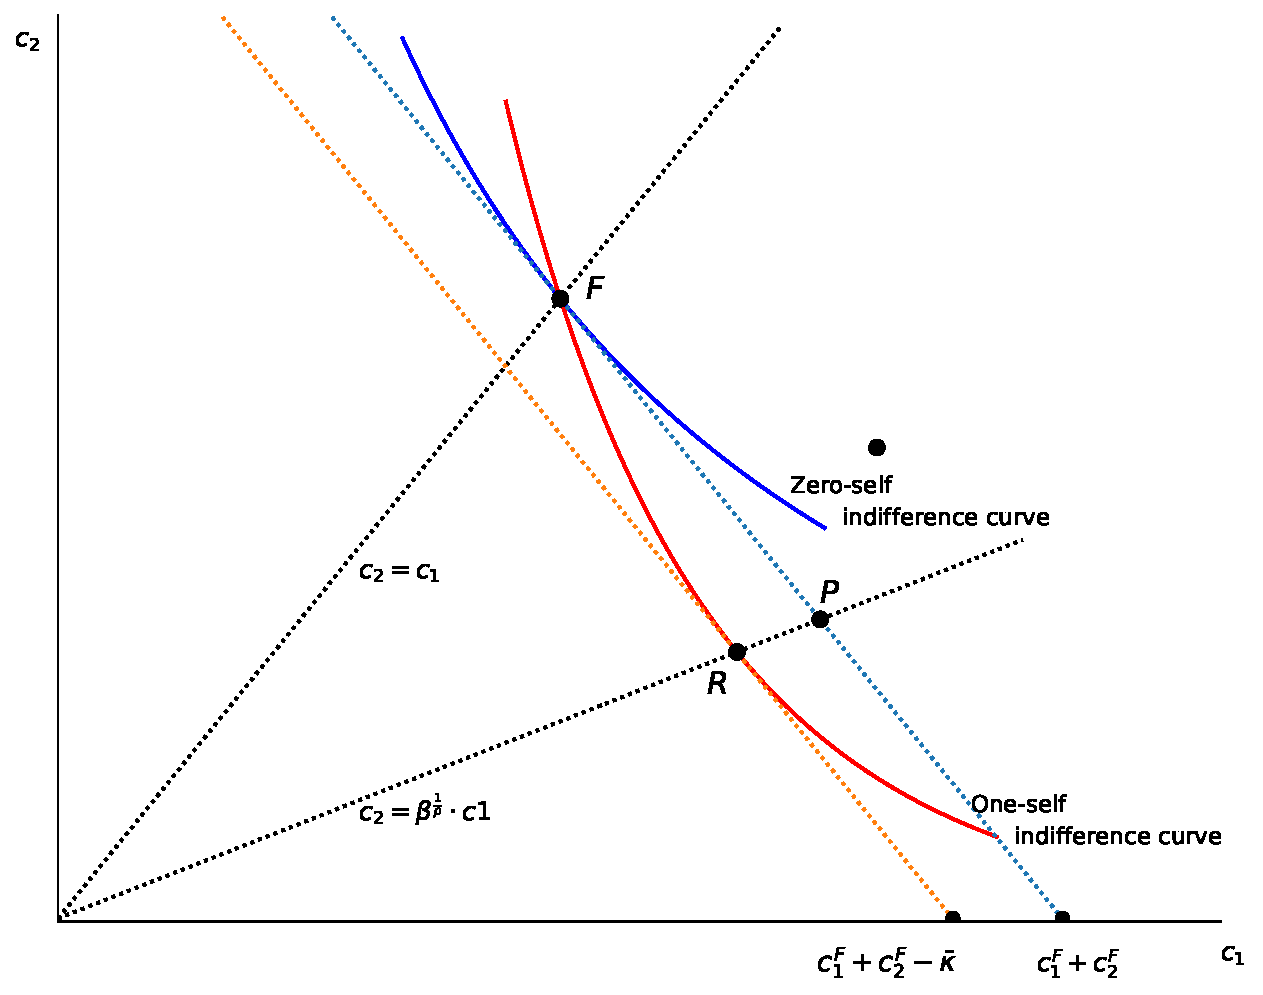
\includegraphics[scale=0.6]{Figure1.pdf}
  \caption{Optimal competitive contract and renegotiation threat}
  \label{fig:c1c2}
\end{figure}


\subsection{Renegotiated contracts}

To derive a no-renegotiation constraint we must understand the
terms of renegotiated contracts even if, in equilibrium, no renegotiations
will take place. Consider a contract $C_{0}^{0}=(c_{0}^{0},c_{1}^{0},c_{2}^{0})$
and the period 1 subgame determined by its associated continuation
contract $C_{1}^{0}=(c_{1}^{0},c_{2}^{0})$. A renegotiation takes
place when One-self and a bank agree to replace continuation contract
$(c_{1}^{0},c_{2}^{0})$ by a new contract $\left(c_{1}^{1},c_{2}^{1}\right)$.

First consider the case when period 1 banks compete to replace contract
$C_{1}^{0}$ with renegotiated contract $C_{1}^{1}(C_{1}^{0})$. The
contract renegotiation problem becomes: 
\begin{align}
C_{1}^{1}(C_{1}^{0}) & =\text{arg max}\ U_{1}(C_{1})\\
s.t. & \ \Pi_{1}(C_{1};C_{1}^{0})\ge\kappa\label{eq:PiGain}
\end{align}
{}where the bank participation constraint (\ref{eq:PiGain}) can be stated
as $(c_{1}^{0}+c_{2}^{0})-(c_{1}+c_{2})\ge\kappa$. To entice a bank
to participate the renegotiated contract must reduce contract expenses (increase bank profits) by an amount that equals or exceeds the
renegotiation cost. Competition insures this constraint exactly
binds. We can solve for an
interior competitive renegotiation contract $C_{1}^{1}(C_{1}^{0})$ using the first-order condition $u'(c_{1}^{1})=\beta u'(c_{2}^{1})$
and binding condition (\ref{eq:PiGain}).\footnote{ For CRRA utility, the contract will be renegotiated to $c_{1}=\frac{c_{1}^{0}+c_{2}^{0}-\kappa}{1+\beta^{\frac{1}{\rho}}}$
and $c_{2}=\beta^{\frac{1}{\rho}}c_{1}$ } For example, with zero renegotiation costs ($\kappa=0$) contract
$F$ in Figure \ref{fig:c1c2} would be renegotiated to $P$. For
positive $\kappa$ (but less than $\bar{\kappa}$ in the figure) the
consumer will surrender just enough surplus to the bank as to get
them to participate, resulting in a contract that lies between $P$
and $R$.

If a bank is a monopolist in period 1, and $\kappa$ is not so high
as to make renegotiation infeasible, the bank's preferred renegotiated contract would
solve:

\begin{align}
C_{1}^{1m}(C_{1}^{0}) & =\arg\max_{C_{1}}\ \Pi_{1}(C_{1};C_{1}^{0})-\kappa\\
\text{s.t.} & \ U(C_{1})\geq U(C_{1}^{0})\label{eq:ugain}
\end{align}
In Figure \ref{fig:c1c2} the monopolist would renegotiate contract
$F$ to a point just \textit{above }$R$ to entice One-self
to participate, captures (practically) all the gains to renegotiation for the
monopolist. Appendix equation (\ref{eq:m-r}) shows the monopolist's
preferred renegotiated contract for any continuation contract
$C_{1}^{0}$.

These renegotiations will not happen in equilibrium but are needed
to determine the path of equilibrium play.

 
\begin{figure}[p]
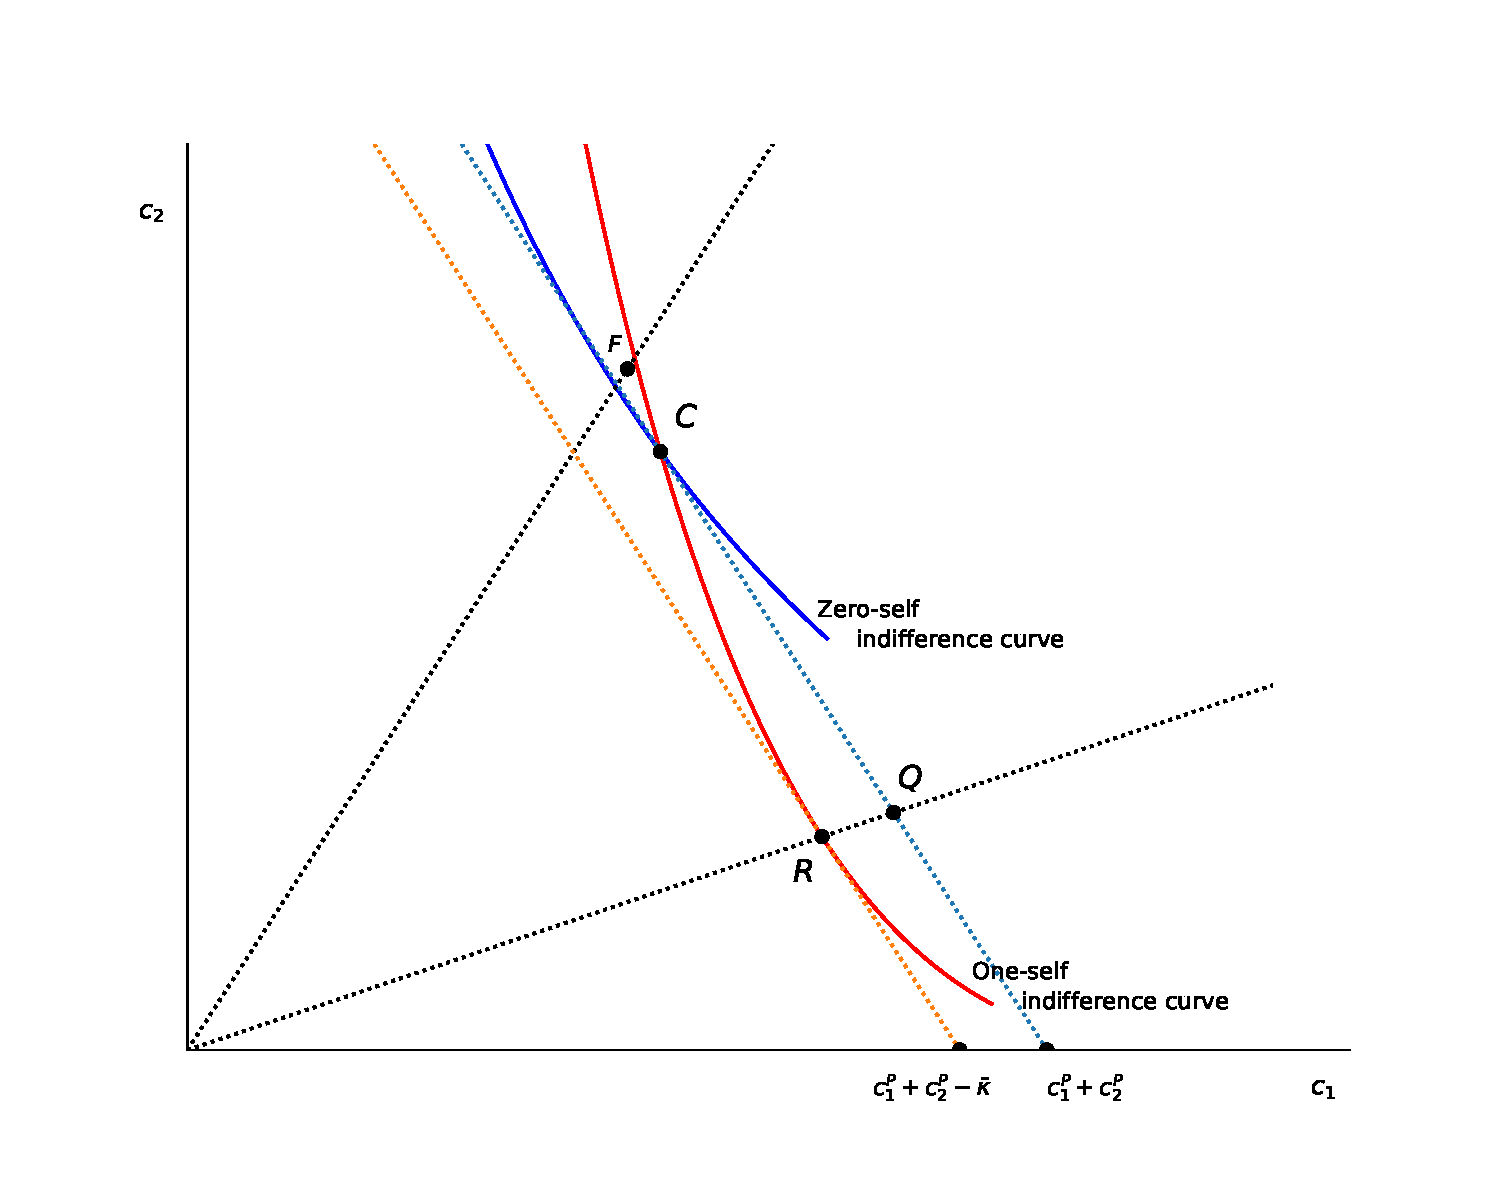
\includegraphics[scale=0.6]{Figure2.pdf}\caption{The no-renegotiation constraint}
\label{fig:renegproof} 
\end{figure}


\subsection{The `no-renegotiation' condition}

\label{sec-no-reneg-cond}

When will a contract \textit{not} be renegotiated in period 1? Assuming
a tie-breaking rule in favor of Zero-self's preferences, depending
on whether the market structure in period 1 is monopolized or competitive,
respectively, the conditions for no renegotiation in period 1 can be described by:
\begin{align}
U_{1}\left(C_{1}^{1}\left(C_{1}^{0}\right)\right) & \leq U_{1}\left(C_{1}^{0}\right)\label{eq:no-reg-comp}\\
\Pi_{1}\left(C_{1}^{1m}\left(C_{1}^{0}\right);C_{1}^{0}\right) & \leq\kappa\label{eq:no-reg-monop}
\end{align}

In fact these two conditions express the same thing: a period
0 contract will be renegotiation-proof if and only if it is \textit{not}
possible in period 1 for a bank and One-self to agree to a new contract
that simultaneously (a) leaves One-self with at least as much discounted
utility as the original contract, and (b) generates a profit gain
of at least $\kappa$ to the bank. In short, the contract will be renegotiation-proof
as long as renegotiation costs are large enough to exhaust any potential
gains to trade between the two parties. These requirements can be
expressed as a single no-renegotiation condition. For the CRRA case:

\begin{align}
u(c_{1}^{0})+\beta u(c_{2}^{0})\ge u\left(\frac{c_{1}^{0}+c_{2}^{0}-\kappa}{1+\beta^{\frac{1}{\rho}}}\right)(1+\beta^{\frac{1}{\rho}})\label{ineq:noreg}
\end{align}

The determination of the boundary between renegotiation-proof and
non-renegotiation proof contracts in $c_{1}-c_{2}$ space is illustrated
in Figure \ref{fig:renegproof}. Consider a candidate continuation
contract $(c_{1}^{0},c_{2}^{0})$ such as at point $C$. One-self
would renegotiate this to any contract lying above their indifference
curve running through $C$. The bank, however, will only agree to a
proposed renegotiation if it can lower contract costs to below existing
costs net of the renegotiation cost $\kappa.$ In diagram terms, the
bank will agree only if the renegotiated contract falls \textit{below}
the lower of the drawn isocost lines with period 1 cost $c_{1}^{0}+c_{2}^{0}-\kappa$.
Contract $C$ is renegotiation-proof because even the most
generous renegotiation that One-self can offer the bank (contract
$R$) falls just short of raising the banks profits by enough to compensate for renegotiation costs. Contract $F$, which smooths consumption
efficiently between period 1 and period 2 under Zero-self's preferences,
is not renegotiation-proof for the given renegotiation cost $\kappa$
illustrated in the earlier Figure \ref{fig:c1c2}. Contract $F$ only becomes renegotiation-proof if external renegotiation costs
rise to $\bar{\kappa}$ or larger, a threshold we determine 
in the next section. 

The no-renegotiation constraint (for a given $\kappa$) is indicated
in Figure \ref{fig:renegproof}. Contracts that are renegotiation-proof must lie below this constraint. The boundaries are described
by a binding equation (\ref{ineq:noreg}).\footnote{From  an examination of the no-renegotiation constraint
(\ref{ineq:noreg}) it is clear there are, in fact, two non-linear boundaries that satisfy this condition. However, given any curvature in \(u(c), \text{ } \)the upper boundary must always bind first, so this is the one we depict and focus on.
When $\kappa=0$ the region coincides with the $c_{2}=\beta^{\frac{1}{\rho}}$
line. See online appendix.} When the no-renegotiation
constraint binds in our profit or utility maximization problem, the
bank must offer a contract along this boundary.\footnote{Recall that by assumption ties are broken in favor of Zero-self's
preferences so no-renegotiation is weakly preferred here. } 

We can now turn back to the period 0 optimization
problem. When that market is competitive the optimal contract (given
any $\kappa$) will be determined by the maximization problem described
by Zero-self's objective (\ref{eq:cobj0}) subject to both the bank
participation constraint (\ref{eq:BPC0}) and no-renegotiation constraint
(\ref{ineq:noreg}). When the market for period 0 contracts is monopolized
the bank maximizes (\ref{eq:monop-obj}) subject to Zero-self's participation
constraint (\ref{eq:BPC0}) and the same no-renegotiation constraint
(\ref{ineq:noreg}). We study these problems in section \ref{sec:imperfectK}
below.

\subsection{Threshold external renegotiation costs }

What is the minimum renegotiation cost sufficient to deter the renegotiation
of a full-smoothing commitment contract? This can be found by setting $c_{1}^{0}=c_{1}^{F}=c_{2}^{0}$
in the no-renegotiation condition (\ref{ineq:noreg}) and solving
for $\kappa$. A competitive full-smoothing commitment contract will
survive if and only if 
\begin{equation}
\kappa\geq\bar{\kappa}\equiv c_{1}^{F}\cdot\Upsilon\label{eq:kbar}
\end{equation}
while a monopolistic full-smoothing commitment contract will survive
if and only if: 
\begin{equation}
\kappa\geq\bar{\kappa}^{m}\equiv c_{1}^{mF}\cdot\Upsilon\label{eq:kbarM}
\end{equation}
where $\Upsilon$ is the constant in (\ref{eq:upsilon}).

Here $\bar{\kappa}$ and $\bar{\kappa}^{m}$ are the threshold minimum
renegotiation costs required to deter the renegotiation of the first-best
efficient smoothing commitment contract. The greater the consumption
levels in the efficient contract (the greater the scope for profitable
contract rearrangements in period 1), the more costly it becomes to
deter renegotiation.
Under competition $c_{1}^{F}$ is independent of autarky utility (given
a fixed value of $y$) so $\bar{\kappa}$ does not depend on how close
or far from optimal consumption smoothing the consumer is in autarky.
With monopoly in period 0 the threshold $\bar{\kappa}^{m}$ which
rises linearly with $c_{1}^{mF}$ will be increasing in autarky utility
$U_{0}^{A}$ (see \ref{eq:c-mf}). Since $c_{1}^{F}>c_{1}^{mF}$ for
any initial $Y_{0}$ we must also always have $\bar{\kappa}^{m}<\bar{\kappa}$.
Proposition 1 summarizes: 
\begin{prop}
\label{Prop:full-commit} Given renegotiation cost thresholds  $\bar{\kappa}$
and $\bar{\kappa}^{m}$ as defined by \ref{eq:kbar} and
\ref{eq:kbarM}. 
\begin{description}
\item [{(a)}] The competitive full-smoothing commitment contract survives
if and only if $\kappa\geq$$\bar{\kappa}$. 
\item [{(b)}] The monopolistic full-smoothing commitment contract survives
if and only if $\kappa\geq$$\bar{\kappa}^{m}$ with $\bar{k}^{m}$
strictly rising in the consumer's autarky utility. 
\item [{(c)}] $\bar{\kappa}^{m}<\bar{\kappa}$. 
\end{description}
\end{prop}
An implication of statement (b)  is that under
monopoly, consumers with better autarky options are less likely to
get full-smoothing commitment contracts. A
consumer with higher autarky utility must be offered higher consumption
by the monopolist, and the no-renegotiation condition is harder to
satisfy at higher levels of consumption. This  dampens the
advantages of improved outside options for sophisticated hyperbolic
discounters contracting with monopoly banks.

A monopolist is relatively better at delivering efficient-smoothing
commitment contracts than under competition ($\bar{\kappa}^{m}<\bar{\kappa}$),
but this is not because monopolists are inherently better at committing;
this follows from the fact that having at the outset extracted
surplus by offering the consumer a contract with the lowest possible
consumption, there is relatively less surplus left to be captured
via renegotiation in period 1.\footnote{There may be other reasons outside of this model that make monopolists
better at committing (i.e. having a higher $\kappa$). Our point is
that this is not necessary for monopolists to offer better smoothing
in more circumstances than competitive firms.}

\section{Constrained Commitment Contracts }

\label{sec:imperfectK}

When bank renegotiation costs are not high enough to sustain efficient-smoothing
commitment contracts, that is where $\kappa<\bar{\kappa}$ under competition
or $\kappa<\bar{\kappa}^{m}$ under monopoly, commitment or renegotiation-proofness
will require contract distortions which we now characterize.

A bank that contracts with naifs will capitalize on the consumer's
failure to anticipate harmful future renegotiations (Section 4.3).
A sophisticated consumer is wise to the problem and will only agree
to renegotiation-proof contracts (Sections 4.2 and 4.3). In the absence
of sufficiently high external renegotiation penalties however the
parties will resort to additional endogenous enforcement mechanisms
by shifting the terms of continuation contracts closer to One-self's
preferred choices as a costly strategy to reduce the gains to renegotiation.
We label these `imperfect-smoothing commitment' contracts. They are
still technically `full commitment' contracts in the sense that renegotiation
is avoided in equilibrium but they generally provide less than perfect
or efficient consumption smoothing from Zero-self's perspective compared
to contracts with stronger external enforcement penalties.

For expositional convenience, we first discuss the monopoly case.

\subsection{Monopoly}

When the market for period 0 contracts is monopolized the bank will
want to maximize multi-period profits subject to Zero-self's participation
and the no-renegotiation constraint

\begin{align}
\max_{C_{0}} & \ \Pi_{0}\left(C_{0};Y_{0}\right)\\
s.t. & \ U_{0}\left(C_{0}\right)\geq U_{0}^{A}\\
 & \ \Pi_{1}\left(C_{1}^{1}\left(C_{1}\right);C_{1}\right)\leq\kappa\label{eq:rpc-m}
\end{align}

A consumer rationally anticipates how her later self may be tempted
to renegotiate and will insist on renegotiation-proofness. When $\kappa<\bar{\kappa}^{M}$
however this will imply distortion away from efficient smoothing which
can only harm bank profits since this raises the contract cost of
keeping the consumer at their reservation utility. Hence the monopoly
bank itself will insist on renegotiation-proof contracts and, as we
shall see, may be willing to spend to improve externally imposed renegotiation
penalties.

The bank wants to search for the most profitable renegotiation-proof
contract that lies on Zero's participation constraint (\ref{eq:CPC0}).
Consider a candidate level of period 0 consumption $c_{0}^{0}$. The
associated continuation contract $C_{1}^{0}$ must lie along Zero-self's
autarky utility surface which can be projected as indifference curve
$\beta\left[u(c_{1}^{0})+u(c_{2}^{0})\right]=U_{0}^{A}-u(c_{0}^{0})$
in $c_{1}-c_{2}$ space. Let this be represented by Zero-self's indifference
curve in Figure \ref{fig:renegproof}. Note this indifference curve
shifts down or up as we increase or decrease $c_{0}^{0}$, which for
the moment we take as given. Many continuation contracts are both
renegotiation-proof and satisfy Zero-self's participation (all in
the area above the indifference curve and below the no-renegotiation
boundary) but the most profitable amongst these will be at point $C$
in Figure \ref{fig:renegproof} at the intersection of the two constraints.
This gives us the optimal renegotiation-proof continuation contract
$C_{1}^{m}(c_{0}^{0})$ from any $c_{0}^{0}$. The monopolist's optimal
contract is then determined by choosing over $c_{0}^{0}$.

\subsubsection{Properties of the contract}

\label{sec_contract_properties}

The renegotiation-proof contract can be explicitly derived for the
CRRA case of $\kappa=0$ (Equation \ref{eq:zerokappa-monop}). For,
$0<\kappa<\bar{\kappa}^{m}$, the contract cannot be derived in closed
form because there are two points where the participation constraint
and no-renegotiation constraint are satisfied with equality (at the
upper and lower boundaries of the set of renegotiation-proof contracts).
However, the key properties of the equilibrium contract can be established
and it can be easily solved for numerically.
\begin{prop}
Suppose $\kappa<\bar{\kappa}^{m}$ and the consumer is sophisticated.
Under monopoly, the profit-maximizing renegotiation-proof contract
($C_{0}^{mP}$) has the following properties:

(i) $\Pi_{0}\left(C_{0}^{mP};Y_{0}\right)<\Pi_{0}\left(C_{0}^{mF};Y_{0}\right)$

(ii) $c_{0}^{mP}>c_{0}^{mF}$ 
\end{prop}
Proposition 2 compares the renegotiation-proof contract to the full-smoothing
commitment contract when the renegotiation-proofness constraint binds.
First, bank profits will be lower than under full-smoothing commitment.
The bank wishes it could promise to not renegotiate but it cannot
make such a promise credible without giving up some profits. The monopolist
would be better off with higher external renegotiation penalties since
in equilibrium renegotiation does not take place.

A related observation is that the bank will prefer not to contract
with individuals who have minimal smoothing needs; for individuals
whose autarky utility is close enough to $U_{0}^{F}$, the bank would
make negative profits under the best renegotiation-proof contract,
so there will be lost trade.

The second statement of the proposition is about the terms of the
contract \textendash{} when full-smoothing commitment is not feasible,
the renegotiation-proof contract will involve higher consumption in
period 0 (i.e. either a smaller loan or less savings) compared to
full-smoothing commitment. The following is a sketch of the argument
(the proof in the appendix uses some additional notation for logical
clarity which we describe intuitively here).\footnote{If the reader prefers to skip this, we present a purely intuitive
explanation of the results near the end of Section 4.2.2.}

Any contract $C_{0}$ can be fully described in terms of three variables,
$c_{0}$, $s$, and $\alpha$. Here, $c_{0}$ is period 0 consumption
and $s$ is the total consumption allocated to periods 1 and 2. $\alpha$
determines the share of $s$ that is consumed in period 1. So, $C_{0}=\left(c_{0},\alpha s,\left(1-\alpha\right)s\right)$.
This notation serves two purposes. First, $\alpha$ captures renegotiation
concerns. Under full-smoothing, $\alpha=\frac{1}{2}$, as this is
optimal from Zero-self's perspective. When the no-renegotiation constraint
binds, we get a function $\alpha\left(s\right)$ which tells us how
much larger $c_{1}$ must be relative to $c_{2}$ so that further
renegotiation would be unprofitable (\ref{eq:alpha-1}). As total
consumption in periods 1 and 2 $s$ rises the parties must rely more
on distorting self-enforcement mechanisms to supplement the fixed
no-renegotiation penalty $\kappa$ as a sufficient deterrent to renegotiation.
Zero-self must in effect become more accommodating of One-self's preferences
so period 1 must get a bigger share. This is indicated by the shape
of the upper boundary of the set of renegotiation-proof contracts
in Figure \ref{fig:renegproof}.

Define the continuation utility from Zero-self's perspective as $V\left(s,\alpha\right)\equiv\beta\left[u\left(\alpha s\right)+u\left(\left(1-\alpha\right)s\right)\right]$.
At any contract that constitutes an optimum, the following must be
true: 
\begin{equation}
\frac{du\left(c_{0}\right)}{dc_{0}}=\frac{dV}{ds}\label{eq:foc-newnotation}
\end{equation}
Otherwise, the bank could raise profits by reallocating consumption
from period 0 to the future or vice versa. This is just a restatement
of the first-order condition.

Now suppose the optimal renegotiation-proof contract specified the
same level of period 0 consumption as the full-smoothing contract,
so $c_{0}^{mP}=c_{0}^{mF}$. Since any future consumption must be
split unevenly, in order to continue to satisfy the consumer's period
0 participation constraint, it must be true that $s^{mP}>$$s^{mF}$.
We show in the appendix that $s^{mP}$ would have to be large enough
that, at these values, 
\begin{equation}
\frac{du\left(c_{0}^{mP}\right)}{dc_{0}}>\frac{dV}{ds}
\end{equation}
so this contract could not be profit-maximizing. In other words, a
switch from full-smoothing commitment to renegotiation-proofness while
maintaining the same $c_{0}$ would require such a large jump in future
total consumption (to continue satisfying Zero-self's participation
constraint) that the marginal utility of future consumption would
be low. So the bank could do better by raising period 0 consumption
at the expense of future consumption.

The bank limits renegotiation possibilities by transferring consumption
away from the future (when renegotiation is a temptation) to the present.
Relative to full-smoothing commitment, consumers get contracts with
larger loans or less savings.

\subsection{Competition}

When the market for period 0 contracts is competitive the optimal
contract solves:

\begin{align}
\max_{C_{0}} & \ U_{0}\left(C_{0}\right)\tag{\ref{eq:cobj0}}\\
\text{s.t.} & \ \Pi_{0}\left(C_{0};Y_{0}\right)\geq0\tag{\ref{eq:BPC0}}\\
 & \ \Pi_{1}\left(C_{1}^{1}\left(C_{1}\right);C_{1}\right)\leq\kappa\tag{\ref{eq:no-reg-monop}}
\end{align}

As noted in section \ref{sec-no-reneg-cond}, the no-renegotiation
constraint \ref{eq:no-reg-monop} assures that gains-to-trade from
renegotiation fall short of bank renegotiation costs. Even if new
banks could enter in period 1 to offer part or or all of the surplus
from renegotiation to One-self in period 1 the constraint deters renegotiation
as long as those banks also face renegotiation cost $\kappa$.\footnote{Later we discuss the empirically relevant cases where competing banks
might enter in period 1 and offer to renegotiate at lower or zero
renegotiation cost).}

We can reuse Figure \ref{fig:renegproof} to interpret the contract
design. Zero-self wants to search for the most profitable renegotiation-proof
contract that lies on the bank's participation constraint (the outer
budget line). Suppose Zero-self has chosen a candidate period 0 level
of consumption $c_{0}^{0}$. To be part of an optimum renegotiation-proof
contract Zero-self must ensure that the continuation contract is renegotiation
proof and satisfies the bank's zero-profit constraint $c_{1}^{0}+c_{2}^{0}=y-c_{0}^{0}$.
Many continuation contracts are both renegotiation-proof and satisfy
the zero-profit constraint (all below both the zero-profit line and
within the no-renegotiation boundary) but the most-preferred by Zero
will be at point $C$ in Figure \ref{fig:renegproof} at the intersection
of the two constraints.\footnote{Note that while we are reusing Figure 2 to describe both the monopoly
and the competitive contract design problem because, conceptually,
they are very similar, optimal consumption levels will be generally
higher under competition so the point $C$ is not the same in both
cases.} This gives us the optimal renegotiation-proof continuation contract
$C_{1}^ {}(c_{0}^{0})$ from any $c_{0}^{0}$. Zero-self's optimal
contract is then determined by backward induction, choosing over $c_{0}^{0}$.

In the special case of perfect competition with costless renegotiation
($\kappa=0$) there will be a unique solution and a closed form. In
figure \ref{fig:renegproof} think of how $C$ slides down the bank's
zero-profit line as $\kappa$ shrinks until we get to a point where
One-self's indifference curve is tangent to the zero-profit line.
This continuation contract is 'renegotiation-proof' only in the very
narrow sense that it won't be renegotiated because it already delivers
One-self's preferred consumption choice. This contract is explicitly
solved in expression (\ref{eq:zerokappa-comp}).

Consider a simple example: with $\beta=0.5$
and $\rho=1$ and $\kappa=0$ the best available competitive contract
$C_{0}^{P}=(150,100,50)$ offers considerably less consumption smoothing
in later periods compared to the benchmark full-smoothing $C_{0}^{F}=(150,75,75)$.
Supose the initial income stream were arranged as $Y_{0}=(100,100,100).$
We  could then interpret the absence of commitment case ($\kappa=0$) as
rolling over of debt that Zero would have preferred to have
seen evenly repaid in period 1 and 2. Instead the entire burden of the debt that Zero took out in period
0 falls due in period 2. Had the income stream
instead started as $Y_{0}=(200,50,50)$ then we might interpret the consumer
in period one as `raiding savings' in period 1 that, with commitment, Zero-self
would have preferred protected for period 2 consumption.

\subsubsection{Properties of the contract}

Suppose contract $C_{0}^{P}$ is the solution to the maximization
problem described by \ref{eq:cobj0}, \ref{eq:BPC0} and \ref{eq:no-reg-monop}. 
\begin{prop}
Suppose $\kappa<\bar{\kappa}$ and the consumer is sophisticated.
The competitive renegotiation-proof contract that
maximizes Zero-self's discounted utility ($C_{0}^{P}$) has the following
properties:

(i) $U_{0}\left(C_{0}^{P}\right)<U_{0}\left(C_{0}^{F}\right)$

(ii) The relationship between $c_{0}^{P}$ and $c_{0}^{F}$ is ambiguous.
There is some $\hat{\rho}$ such that: if $\rho\leq\hat{\rho}$, then
$c_{0}^{P}>c_{0}^{F}$; if $\rho>\hat{\rho}$, then there are parameter
values under which $c_{0}^{P}<c_{0}^{F}$. 
\end{prop}
The first statement is straightforward: Since $\kappa<\bar{\kappa}$
means the new renegotiation-proofness constraint (\ref{eq:no-reg-monop})
binds full-smoothing smoothing cannot be achieved and the consumer's
welfare must be lower than under the first-best contract.

The second statement regards whether period 0 consumption  (and hence period 0 net-borrowing) will be higher or lower compared to the full-smoothing
commitment? The proposition is that this depends on the intertemporal elasticity of substitution $\frac{1}{\rho}$.
Following the modified notation of Section \ref{sec_contract_properties}
and first-order condition (\ref{eq:FOC_comp}),  the following must be true of the competitive full-smoothing commitment contract $C_{0}^{F}$:

\begin{equation}
\frac{du\left(c_{0}^{F}\right)}{dc_{0}}=\frac{dV\left(s^{F},\frac{1}{2}\right)}{ds}
\end{equation}

Now suppose the competitive renegotiation-proof contract $C_{0}^{P}$
involves the same period 0 consumption as under full-smoothing commitment,
so that $c_{0}^{P}=c_{0}^{F}$. By the bank's zero-profit constraint,
the contract will also have $s^{P}=s^{F}$, but consumption will now be
split in period 1's favor. If the utility function is relatively linear
(low $\rho$), then an imbalanced split of $s$ results in a lower
marginal utility than from a balanced split. So: 
\begin{equation}
\frac{du\left(c_{0}^{F}\right)}{dc_{0}}>\frac{dV\left(s^{F},\alpha\left(s^{F}\right)\right)}{ds}
\end{equation}

In such a case, the renegotiation-proof contract must involve higher
period 0 consumption than the full-smoothing commitment contract.

If, on the other hand, the utility function is highly concave (high
$\rho$), then an unbalanced split results in higher marginal utility
relative to full-smoothing. In such cases, the renegotiation-proof
contract will adjust to lower period 0 consumption compared to full-smoothing
commitment.\footnote{The  cutoff value $\hat{\rho}$ is somewhat
complicated, as $\frac{dV}{ds}$ depends not just on $u'\left(c_{1}\right)$
and $u'\left(c_{2}\right)$, but also on how the sharing rule, $\alpha\left(s\right)$,
changes with $s$.} This can be seen clearly for the case of $\kappa=0$ where from the closed form expression for \(c_0^P\) (equation
\ref{eq:zerokappa-comp}) we can show  \(c_{0}^{P} \gtrless c_{0}^{F} \) as \(\rho \lessgtr 1\).

So, under competition, a binding no-renegotiation constraint can
change the contract in either direction: a larger period zero loan (less saved)
or a smaller loan (more saved). Period 2 consumption however always
falls relative to the full-smoothing commitment case, even in the
cases when Zero-self saves more/borrows less. In fact for CRRA utility
the adjustment of period 0 consumption (in the absence of commitment
compared to with commitment) is always relatively small while the
adjustment to period 1 and period 2 consumption is proportionately much
larger.\footnote{To illustrate, with $\kappa=0$ at no point does period 0 consumption
rise or fall by more than six percent for any value $\rho\in(0,\infty)$
and $\beta\in(0,1)$ but at reasonable parameter values such as $\rho=0.5$
and $\beta=0.5,$  period 1 consumption
rises almost 50 percent above the level it would be with commitment, and
period 2 consumption falls to just 37 percent of what it would be.} In other words, and despite having a first-mover advantage, Zero-self
can do little other than to partially accommodate to the consumption
pattern that One-self wants to impose.

The contrast between monopoly and competition can be explained using
the intuition of income and substitution effects. In either case,
a move from full-smoothing commitment can be viewed as a rise in the
``price'' of delivering a unit of future utility from Zero-self's
perspective. As a result, substitution effects will lead to an increase
in period 0 consumption and a drop in future consumption. Under monopoly,
since the consumer is always left at her autarky utility, there are
no income effects. When the renegotiation-proofness constraint binds,
the price of future utility effectively rises, as a result of which
substitution effects lead to greater period 0 consumption. Under competition,
income and substitution effects work against each other; the net result
depends on the shape of the consumer's utility function.\footnote{This intuition applies to CRRA and widely across other standard utility
functions, but there are exceptions. As shown in \citet{basu2020},
it is possible to construct utility functions where even as the overall
price of delivering future utility goes up, at some points the \emph{marginal}
price does not. In such cases, even under monopoly the change in contract
terms from full-smoothing to imperfect-smoothing commitment contract
could be ambiguous.}

\subsection{Contracting with Naive Discounters}

For naive agents, the problem of renegotiation does not generally
lead to a renegotiation-proof contract. The naif believes she will
not be tempted to renegotiate.  Under monopoly, the
bank can add to its profits by engaging in renegotiation that was not
anticipated by the consumer in period 0. Under competition, banks
are led to return the potential surplus from renegotiation to the Zero-self.\footnote{A similar analysis could be carried out if consumers were misinformed
not about their own preferences but about $\kappa$.}

\subsubsection{Monopoly}

Relative to a sophisticated consumer, with a naive consumer the monopolist
bank can make additional profits on two margins. First, since there
is no perceived renegotiation problem, the consumer is willing to
accept a contract that is more profitable for the bank up-front; subsequently,
possible renegotiation generates additional profits for the bank.\footnote{There is an additional consideration \textendash{} that naive hyperbolic
discounters might be inaccurately optimistic about autarky outcomes
because of a failure to anticipate commitment problems. This would
have the interesting effect of tightening the participation constraint
and reducing surplus available to the monopolist}

The bank must choose between a renegotiation-proof contract and one
that will be renegotiated upon. If $\kappa$ is sufficiently large
there is little to gain from renegotiation and the consumer will be
offered the full-smoothing commitment contract. But when $\kappa$
is relatively small, the bank might prefer to offer a contract that
will subsequently be renegotiated. In such cases, the bank solves
the following problem:
\begin{eqnarray}
\underset{C_{0}}{\text{max}} & \ \Pi_{0}\left(C_{0};Y_{0}\right)+\Pi_{1}\left(C_{1}^{m1}\left(C_{1}\right);C_{1}\right)-\kappa\\
s.t. & \ U_{0}\left(C_{0}\right)\geq U_{0}^{A}\label{eq:pc-n}
\end{eqnarray}

Let the solution, denoted $C_{0}^{mN}$, is explicitly derived
in the appendix (\ref{eq:naive-monopolist-contract1}, \ref{eq:naive-monopolist-contract2}).
The bank maximizes profits by offering a contract that divides future
consumption as much in favor of period 2 as possible. The greater
the imbalance between the contracted $c_{1}$ and $c_{2}$, the greater
the bank's profits from renegotiation. We show that if $\rho<1$,
the contract is at a corner solution where $c_{1}=0$. If $\rho>1$,
an explicit solution does not exist, but maximization pushes the contract
to a point where $c_{2}$ approaches infinity.\footnote{This assumes the consumer remains naive even in the face of such an incredible contract. While it is of interest to understand this benchmark case, a more realistic setup would \textbraceleft CITE\textbraceright\ .} This contract can be compared to both the full-smoothing commitment
contract and the renegotiation-proof contract for sophisticates. In
particular, it will involve lower period 0 consumption than under
both full-smoothing commitment and renegotiation-proofness. This result
might appear counter-intuitive. In the case of lending, it does not
reinforce the narrative of banks preying on naive consumers by offering
them relatively large loans with steep repayments. Indeed, there are
other considerations beyond the scope of this model, such as the possibility
of collateral seizure, that could generate large loans. But our limited
model helps to highlight a particular aspect of contracting with naive
hyperbolic discounters: here, the bank offers them relatively \emph{small}
loans because its gains from renegotiation depend on the surplus that
the initial contract delivers to periods 1 and 2. In order to fully
take advantage of the consumer's naivete, the consumer must start
out with sufficiently small repayments that the bank could profit
from rearranging them.

The next proposition summarizes the above discussion. 
\begin{prop}
Suppose the consumer is naive. Under monopoly:

(i) If $\kappa$ is sufficiently higher than $\bar{\kappa}^{m}$,
the firm will offer the agent the full-smoothing commitment contract
($C_{0}^{mF}$) and it will not be renegotiated.

(ii) Otherwise, the contract $C_{0}^{mN}$ will satisfy $c_{0}^{mN}<c_{0}^{mF}<c_{0}^{mP}$
(either explicitly or in the limit), and it will be renegotiated in
period 1. 
\end{prop}

\subsubsection{Competition}

Under competition with naive consumers, contracts must account for
renegotiation to have firms continue earning zero profits. Note that if contracts are not exclusive, the consumer gets offered
the full-smoothing commitment contract, which then gets renegotiated
if $\kappa<\bar{\kappa}$. This is because the firm offering the contract
in period 0 does not expect to benefit from renegotiation, so the
contract gets competed down to the one that maximizes the naive Zero-self's
perceived utility while delivering zero profits to the bank.

Under exclusive contracts, period 0 competition will imply that anticipated profits from future renegotiation
will be returned to the consumer through more favorable initial contracts.
If $\kappa$ is sufficiently small, the equilibrium contract involves
renegotiation and satisfies: 
\begin{align}
\underset{C_{0}}{\mbox{\ensuremath{max}}} & \ U_{0}\left(C_{0}\right)\\
s.t. & \ \Pi_{0}\left(C_{0};Y_{0}\right)+\Pi_{1}\left(C_{1}^{m1}\left(C_{1}\right);C_{1}\right)\geq\kappa
\end{align}

Let the solution be denoted $C_{0}^{N}$as explicitly derived
in the appendix (\ref{eq:naive-comp-contract1} and \ref{eq:naive-comp-contract2}).
As under monopoly, contracts divide future consumption as much in
favor of period 2 as possible to maximize the potential gains
from renegotiation. In the context of loans, this suggests contracts
where the debt burden is heaviest in the intermediate stages, resulting
in renegotiation to postpone payments.

Unlike under monopoly, competition for consumers returns anticipated renegotiation
gains to the consumer. Some of these gains are returned to the Zero-self,
so there is no clear prediction about whether period 0 consumption
will be lower or higher than under full-smoothing commitment. 
\begin{prop}
Suppose the consumer is naive. Under competition:

(a) If contracts are not exclusive: The consumer will accept the full-smoothing
commitment contract, $C_{0}^{F}$. The contract will be renegotiated
in period 1 if and only if $\kappa<\bar{\kappa}$.

(b) If contracts are exclusive: 

\begin{enumerate}
(i) If $\kappa$ is sufficiently higher than $\bar{\kappa}$, the
consumer will accept the full-smoothing commitment contract ($C_{0}^{F}$)
and it will not be renegotiated.

(ii) Otherwise, the consumer will accept a contract $C_{0}^{N}$ with
the following properties: if $\rho<1$, $c_{0}^{N}<c_{0}^{F}$. If
$\rho>1$, then there are parameter values under which $c_{0}^{N}>c_{0}^{F}$. \end{enumerate}
\end{prop}

\section{Commercial non-profits and Hybrid ownership forms}

\label{nonprofits}

Consider now the case of a firm that, in a pre-contract stage, has
the possibility of choosing its ownership structure as a way to tie its own hands. The firm might incorporate
as a legal non-profit or, more broadly, choose a degree of `hybrid'
ownership, for example by retaining for-profit status but actively attracting
social investors to establish considerable equity stakes and managerial
control. Similar to \citet{hansmann1996a} and as discussed
in the introduction, we think of these choices as imposing  restrictions on the firm's
ability to distribute profits to shareholders and managers in ways that can temper incentives: 
\begin{defn*}
Given `raw profits' $\Pi_{0}$, a `nonprofit' firm retains `captured
profits' $f\left(\Pi_{0}\right)$, where $f\left(0\right)=0$, $f'\left(\Pi_{0}\right)\in\left(0,1\right)$,
and $f''\left(\Pi_{0}\right)\leq0.$ 
\end{defn*}
This formulation follows \citet{glaeser2001} who argued that although
the principals of a non-profit might technically be legally barred from
tying their own compensation to cash profits, in practice they often can capture a
fraction of those profits  imperfect and costly ways via the consumption
of perquisites or `dividends in kind' (e.g. the lavish expense account).
The shape of \(f\) captures the idea that the ability to employ perquisites and other such methods to substitute for unrestricted consumption
falls with profits.

Setting aside mission or tax-advantage concerns that might additionally drive firms to adopt nonprofit
or hybrid status, we examine when purely profit-minded firms might
make such strategic governance choices; i.e. when a voluntary restriction
on their ability to distribute profits will make a self-interested firm better
off?\footnote{Indeed, welfare concerns could directly improve consumer outcomes
by either allowing Zero-self's participation constraint to be slack
or by raising the costs of renegotiation $\kappa$. We consider the
latter point in an example below.} This has parallels to the explanation for commercial nonprofits due
to \citet{hansmann1996a} and modeled by \citet{glaeser2001} but
established on quite different behavioral grounds.\footnote{In those  accounts a firm delivers less than a promised quantity or
quality of a good or service, unambiguously harming the time-consistent
client. The client discovers this after the fact but cannot challenge
the contract breach only because it is too difficult or costly. In
contrast in our model the firm and the One-self customer both gain
from voluntarily breaking existing contract commitments and Zero-self
is no longer around to mount a challenge.}

At the outset, note that profit-oriented principals
have no incentive to switch to hybrid/nonprofit status when consumers
are naive. Since the consumer perceive no need for commitment,
any promise of superior commitment is of no value to her. 

With sophisticated consumers a firm, established as a commercial non-profit, may have  an opportunity to extract greater surplus
from the consumer (by providing commitment), but now faces restrictions
on the ability to distribute this surplus to managers and shareholders.
This trade-off is sensitive to market structure. Under competition,
a lender's ability to provide effective commitment through non-profit
status depends on the exclusivity of contracts. When long-term contracts
can be made exclusive, the tradeoff disappears and all active firms
function as non-profits to attract customers. If other firms are for-profit,
a firm could make positive profits by offering superior commitment
as a non-profit (this is valuable even if its enjoyment of these profits
is limited).
In equilibrium all firms switch and since they are earning zero profits, there is no cost to retaining non-profit status.

When contracts cannot be made exclusive, commitment generated through non-profit
status becomes impossible to achieve. Each firm now has an incentive to switch to
for-profit status in period 1 to take advantage of the opportunity to re-finance
\textit{other} banks' loans. As a result, for-profit firms must be
active in equilibrium, and their presence will eliminate the possibility
of non-profit commitment in period 0.

This might, for example, help explain a key difference between early microfinance
where  larger non-profit 
firms tended to dominate\ (e.g. Grameen Bank of Bangladesh, BRI Indonesia) offering rigid multi-period contracts, and say competitive
commercial credit card lending, or more competitive microfinance, which offer greater refinancing flexibility
(credit card punishments gain salience because they are\textit{ less}
(not more)\ strict, and therefore frequently triggered).

\subsection{Monopoly}

In a pre-contract phase the firm  establishes its type via
the adoption of legal non-profit status and/or by choosing stable and credible
ownership and governance structures that commit it to profit distribution
limitations. If the monopoly firm were to operate as a nonprofit or
a hybrid (adopt \( f\)), when facing a sophisticated hyperbolic discounter it would
design a renegotiation-proof contract to solve: 
\begin{align}
\underset{C_{0}}{\text{max}} & \ f\left(\Pi_{0}\left(C_{0};Y_{0}\right)\right)\\
\text{s.t.} & \ U_{0}\left(C_{0}\right)\geq U_{0}^{A}\\
 & \ f\left(\Pi\left(C_{0};Y_{0}\right)+\Pi_{1}\left(C_{1}^{m1}\left(C_{1}\right);C_{1}\right)\right)-f\left(\Pi\left(C_{0};Y_{0}\right)\right)\leq\kappa\label{eq:no-reneg-np}
\end{align}

Why operate as a nonprofit
when that reduces its ability to capture profits? The answer lies
in the loosening of the no-renegotiation constraint (\ref{eq:no-reneg-np}).
Now smaller gains from renegotiation are captured compared to the pure for-profit firm. Clearly, the pure for-profit monopolist's contract
($C_{0}^{mP})$ would now leave the now more relaxed no-renegotiation constraint slack.
The non-profit can now offer to credibly commit to not renegotiate
contracts that offer greater consumption smoothing across periods
1 and 2, so Zero-self becomes more willing to pay for these smoother consumption
streams.

The `captured-profits' maximizing solution will be given by a contract that we denote $C_{0}^{mNP}$. If $\kappa<\bar{\kappa}^{m}$, with a relaxed
renegotiation-proof constraint $\Pi_{0}(C_{0}^{mNP};Y_{0})>\Pi_{0}(C_{0}^{mP};Y_{0})$
but whether or not it will be in the bank principals' best interest
to strategically convert to non-profit status depends on whether the
captured profits under non-profit status exceed the profits they could
earn as a pure for-profit, in other words on whether $f\left(\Pi_{0}(C_{0}^{mNP};Y_{0})\right)>f\left(\Pi_{0}(C_{0}^{mP};Y_{0})\right)$.
The monopolist faces a tradeoff in considering non-profit status:
higher raw profits (as the commitment problem is partly solved) but
a diminished capture of those raw profits.

 Proposition 6 (in Section 5.2) establishes the
existence of captured profit functions that would be strictly preferred
to for-profit status for monopoly firms. 
Given particular captured profit functions, we can also ask types of
consumers are more likely to be served by such firms. If
consumers are far from optimal in autarky, then the pure for-profit firm
would make substantial profits. In such cases, the extra surplus from the non-profit's
credibility advantage does not compensate for the  restrictions on profit distributions required.
 However, for consumers with higher autarky utility, we can describe situations where nonprofit or hybrid status firms earn higher captured profts compared to pure for-profits. In some environments, non-profits can operate where pure for-profits would fail to operate profitably at all.
\subsubsection{An example}

Consider a firm that may choose its degree of
hybrid-ness or for-profit orientation, indexed by a parameter $\alpha\in\left[0,1\right]$.
For a chosen $\alpha$, captured profits are a linear function of raw profit:
\begin{equation}
f\left(\Pi_{0}\right)=\alpha\Pi_{0}
\end{equation}

An $\alpha=1$
would represent a pure for-profit investor-led firm, $\alpha=0$ a
strictly regulated non-profit.
We can also allow $\alpha$ to directly affect the non-pecuniary renegotiation
cost the firm's principals incur when they opportunistically break
contractual promises. A more hybrid or non-profit firm
dominated by social investors is more likely to hire staff and managers
that internalize client welfare and social investor motivations and
are hence more likely to feel non-pecuniary costs associated with
guilt, cognitive dissonance, or loss of reputation from breaking promises. If we label the cost of renegotiation $\eta\left(\alpha\right)$ \textendash{}
replacing our earlier $\kappa$ \textendash{} this is captured
by assuming that function $\eta$ falls weakly in $\alpha$. Putting
both mechanisms together gives a modified no-renegotiation constraint: 
\begin{equation}
\alpha\Pi_{1}(C_{1}^{m1}(C_{1});C_{1})\leq\eta(\alpha)\label{eq:no_reneg_np}
\end{equation}
This states that the fraction of raw profits
$\Pi_{1}$ that can be captured from  contract renegotiation must
not exceed renegotiation costs. If we define $\kappa(\alpha)\equiv\frac{\eta(\alpha)}{\alpha}$, this
no-renegotiation constraint can be written as

\begin{equation}
\Pi_{1}(C_{1}^{m1}(C_{1});C_{1})\leq\kappa(\alpha)\label{eq:no-kalpha}
\end{equation}
which looks just like our earlier constraint (\ref{eq:rpc-m}) except $\kappa$
is now a function of $\alpha$. The earlier renegotiation problems
were for the special case of a pure for-profit firm with $\alpha=1$
but we can now analyze how contracting, captured profits, and client welfare
change with ownership/governance choices  $\alpha$  in a strategic equilibrium.

Note that if the loosening of the no-renegotiation constraint
happens primarily via the right-hand side (i.e. via term $\eta\left(\alpha\right)$,
which represents the firm's motivation to honor the initial agreement),
the firm benefits unambiguously\textendash as it is able to offer better
commitment \emph{and} fully retain the added profits.
This suggests that hiring caring, mission-oriented staff might be good for the firm's bottom line -- something that is not generally true in a market with only time-consistent clients. 
\begin{figure}
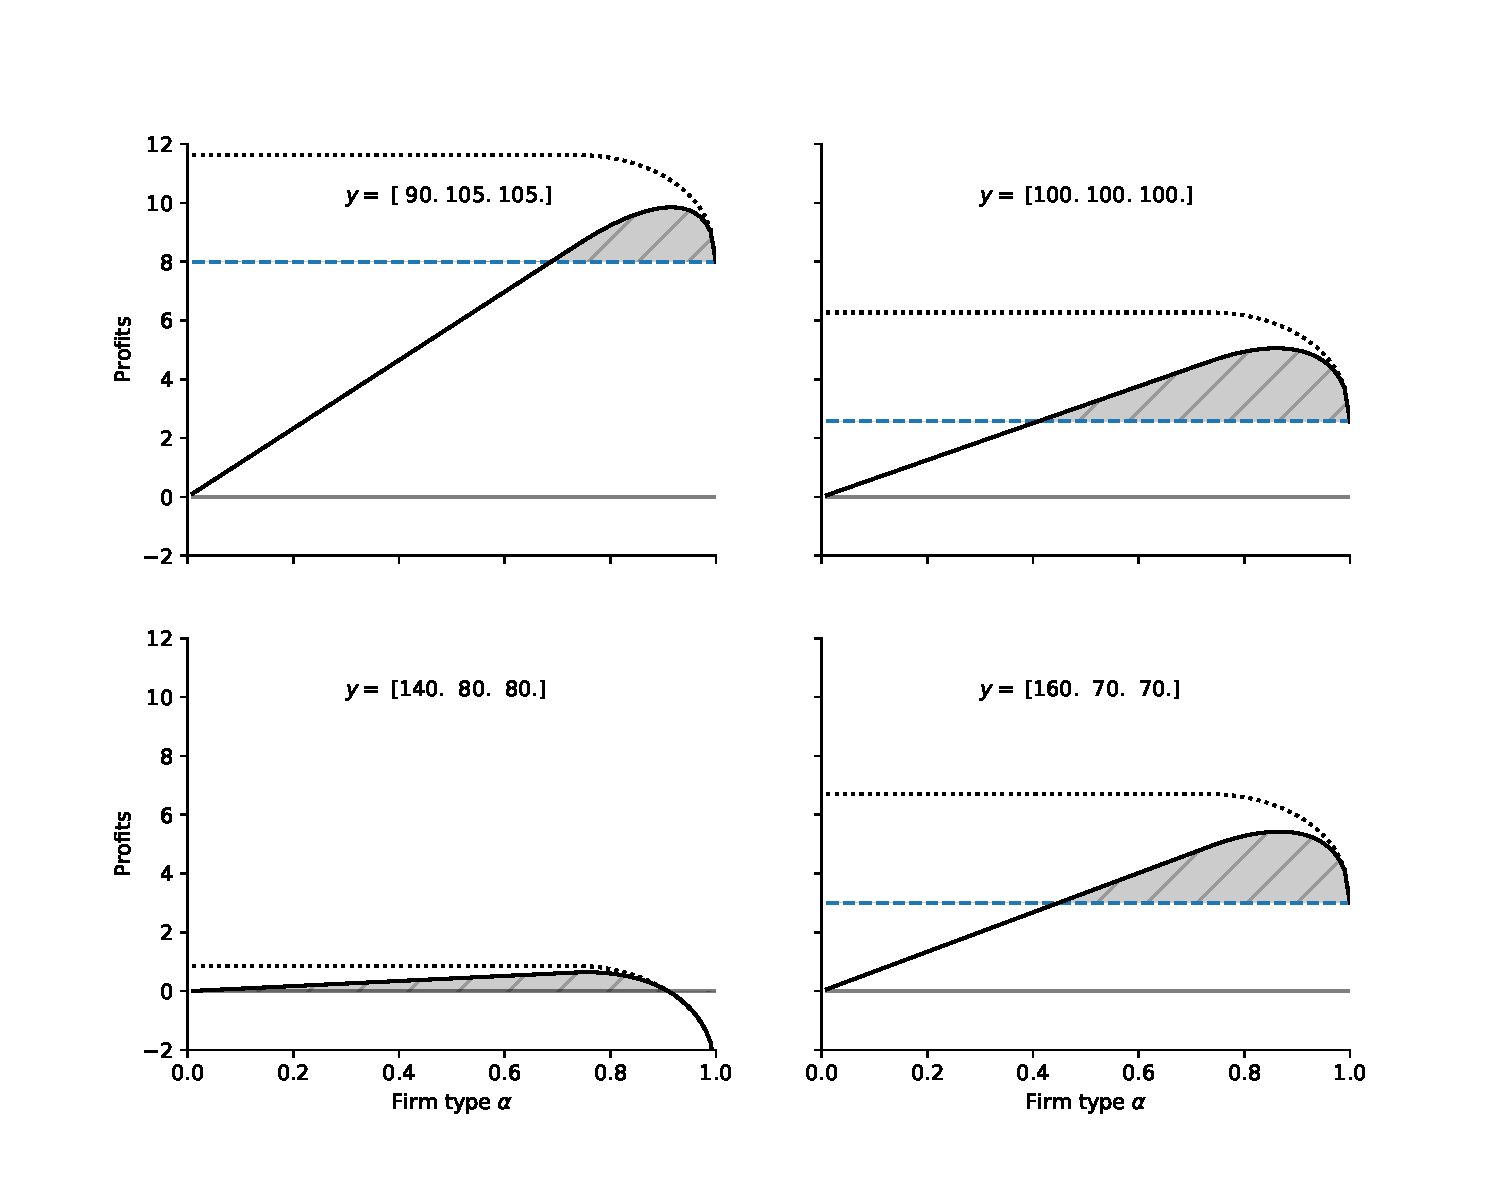
\includegraphics[scale=0.75]{Figure3.pdf}
\caption{\label{fig:nonprofit}Captured rent by ownership status and endowment
income}
\end{figure}

Figure \ref{fig:nonprofit} illustrates cases where non-pecuniary
costs to breaking promises fall with $\alpha$
according to $\eta(\alpha)=10 \cdot (1-\alpha)$ and hence $\kappa(\alpha)=10 \cdot (1-\alpha)/\alpha$.
The subplots show captured profits at different
levels of $\alpha$ for four  different consumer types, differentiated by their initial income streams. In each case \(\beta=0.65\) and $\rho=1.05$ but consumers differ in terms of initial  income streams. All streams have present value of 300
but differ  in terms of period 0 income \(y_{0}\) with remaining income  divided equally between period 1 and 2, so \(y_1=y_2=\frac{300-y_0}{2}\). 
 The higher dotted curved lines in each subplot
represents `raw' profits $\Pi_{0}(C_{0}^{mNP};Y_{0})$ and the lower
solid curve captured profits $\alpha\Pi_{0}(C_{0}^{mNP};Y_{0})$. A horizontal
line has been drawn in to indicate the level of profits $\Pi_{0}(C_{0}^{mP};Y_{0})$
earned by a pure for-profit ($\alpha=1 \text{ and } \kappa (1)=0\)) and the shaded area indicate the extra profits captured by a hybrid firm of type \(\alpha\) compared to that pure-profit benchmark. Consider the top left panel
where the customer has initial income $(90,105,105)$. These  customers want to borrow significantly in period 0 so bank
profits would be large, even under the renegotiation-proof contract offered by the pure for-profit. Hybrid status by lowering $\alpha$ and offering better commitment contracts confers some profit gain.
For really heavy borrowers, with even lower \(y_{0}\) (not depicted), the gain to hybrid status become negligible  and  pure for-profits likely dominate. On the other hand, customers with endowments such as  $(140,80,80)$ are already fairly close
to their preferred consumption stream so the profits to be captured
even under full commitment are not that large. The pure and more for-profit firms can not  earn positive profits but a broad range of non-profits survives.  In a market where consumer demand for savings is higher (bottom right panel) we see  profits climb again and more commercially-oriented firms become more likely to prevail. 

\subsection{Competition}

\subsubsection{Exclusive contracts}

Consider the competitive market situation where contracts can be assumed to remain exclusive, so that any potential renegotiation surplus between the bank and the One-self
goes to the bank.
In this setting, a nonprofit/hybrid firm will be led to offer contract
terms to solve: 

\begin{align}
\underset{C_{0}}{\text{max}} & \ U_{0}\left(C_{0}\right)\\
\text{s.t.} & \ f\left(\Pi_{0}(C_{0};Y_{0})\right)\geq0\\
 & \ f\left(\Pi\left(C_{0};Y_{0}\right)+\Pi_{1}\left(C_{1}^{m1}\left(C_{1}\right);C_{1}\right)\right)-f\left(\Pi\left(C_{0};Y_{0}\right)\right)\leq\kappa\label{eq:no-reneg-enp}
\end{align}

Label the contract that solves this program  $C_{0}^{eNP}$. Consider first a field where all firms start as pure for-profits
and earn zero profits. If the no-renegotiation constraint binds, Zero-self's
utility must be lower than optimal. Starting from this situation consider
now firms' strategic choice to adopt non-profit status.
Any firm that switches into nonprofit status can make positive
profits while offering Zero-self a contract with a higher discounted
utility because of the loosened no-renegotiation constraint (\ref{eq:no-reneg-enp}).
So, if the borrowers are sophisticated hyperbolics, in equilibrium,
all firms become nonprofit and earn zero profits.

\subsubsection{Non-Exclusive Contracts}

Now, assume that exclusivity, or  period 1 monopoly power, disappear.
Firms can compete to renegotiate each other's contracts in period
1.

If there were only non-profits in equilibrium, any one firm could now make
positive profits by switching to for-profit status (or a new firm might enter), undoing a rival
bank's contract in period 1. As a result, equilibrium contracts will be
determined by for-profit firms, and consumers will be offered lower
commitment than from non-profit firms alone.\footnote{The same argument applies if banks can costlessly renegotiate other bank's contracts.} 
The above discussion is summarized: 
\begin{prop}
(a) Suppose $\kappa<\bar{\kappa}^{m}$. Under monopoly, there exist
captured profit functions such that the firm will operate as a nonprofit.

(b) Suppose $\kappa<\bar{\kappa}$. Under competition: (i) If contracts
are exclusive, firms will operate as nonprofits for any captured profit
discount function. (ii) If contracts are not exclusive, there is no
captured profit discount function under which firms will operate as
nonprofits. 
\end{prop}

\section{Discussion}

We discuss three areas of practical and policy concern that the
analysis aims to engage with.

\subsection{Commitment as a form of Consumer Protection}

Concerns about excessive refinancing and `over-indebtedness' have
been raised, especially in the lead up and wake of financial crises.
On the eve of the mortgage banking crisis of 2007, over 70 percent
of all new subprime mortgage loans were refinances of existing mortgages
and approximately 84 percent of these were `cash out' refinances \citep{demyanyk2011}.
In the market for payday loans in the United States economists and
regulatory observers express concern not so much that fees are high
(the typical cost is 15\% of the amount borrowed on a 2 week loan)
but that 4 out of 5 payday loans are `rolled over' or renewed
rather than paid off at maturity, resulting in very high total loan costs and placing
many people into very difficult debt management situations \citep{deyoung2015}.

Consumer protection problems are often analyzed emphasizing two
broad channels: naive or uneducated consumers and their failure to correctly
anticipate fees and punishments (see \citet{gabaix2006},
\citet{armstrong2012}, and \citet{akerlof2015} for related arguments),
and/or bank's moral hazard (see \citet{dewatripont1999} and \citet{oak2010}).
We have argued that, given evidence of time-inconsistent
preferences,\footnote{See, for example, \citet{laibson2003}, \citet{ashraf2006},
\citet{gugerty2007}, and \citet{tanaka2010}.} a bank's ability to provide credible commitment should also fall
under this umbrella \textendash\  sometimes consumers \textit{want} punishments
or fees to limit renegotiation.

In light of consumer credit
market crises, there has been renewed emphasis on consumer protection and
better governance and regulation in banking.\footnote{In the US, the Consumer Financial Protection Bureau was set up in
2011 under the Dodd\textendash Frank Wall Street Reform and Consumer
Protection Act. In India, the far-reaching Micro Finance Institutions
Development and Regulation Bill of 2012 was designed to increase government
oversight of MFIs in response to the credit crisis in the state of
Andhra Pradesh, and the perception that lax consumer protection and
aggressive lending practices had led to rising over-indebtedness and
stress.} One particular outcome of concern has been borrower over-indebtedness,
an issue that has been at the center of recent microfinance repayment
crises in places as far-flung as Morocco, Bosnia, Nicaragua and India,
as well as the 2008 mortgage lending crisis in the United States.
In each of these cases the issue of refinancing or the taking of loans
from multiple lenders emerges.

Journalistic and scholarly analyses of such situations, including
the recent mortgage crisis in the United States, often frame
the issues as problems of consumer protection, suggesting lenders design products to purposefully take advantage of borrowers
who have limited financial literacy skills and are naive about their
self-control problems. Informed by such interpretations, regulations
introduced in the wake of these crises swung toward restricting
the terms of allowable contracts, for example by setting maximum interest
rates and limiting the use of coercive loan recovery methods.

We place consumers' struggles with intertemporal self-control issues
at the center of the analysis, but argue that borrowers may be more
sophisticated in their understanding of their own time-inconsistency
than is often assumed. From this perspective, `predatory lending'
is not primarily about tricking naive borrowers into paying more than
they signed up for with hidden penalties or misleading interest rates
quotes, but about offering excessive flexibility and refinancing of
financial contracts in ways that may undermine the commitments
to long term consumption and debt management paths that borrowers
may want to put in place.\footnote{\citet{bond2009} discuss evidence of predatory lending in the context
of mortgages. In 2016 the Consumer Financial Protection Bureau put
forth a proposal to protect payday loan consumers including limits
on the number and frequency of re-borrowings \citep{cfpb2016}.}

Here, a bank that promises to be rigid and is then flexible could
be seen as hurting, rather than helping, the consumer. We take seriously
the bank's ex-post considerations and derive conditions under which
it would renegotiate.
In this sense, our paper complements some others that demonstrate
how commitment can be undone in related settings. \citet{gottlieb2008}
shows how competition leads to inefficient outcomes in immediate rewards
goods. \citet{heidhues2010} study the mistakes of partially naive
borrowers in competitive credit markets. \citet{mendez2012} analyzes
predatory lending with naive consumers. 

\subsection{Commercial Non-profits and hybrid ownership in Finance}

 Henry
\citet{hansmann1996a} argued that in markets where the
quality of products or services were difficult to verify, clients
would rationally fear that investor-led firms might opportunistically
skimp on the quality of a promised product or service, or reveal a
hidden fee, and this could greatly reduce or even eliminate contracting.
 `Commercial non-profit' status might then be a
costly but necessary strategy by firms to commit to not act opportunistically,
hence enabling trade.
Hansmann used as a primary example the development of
consumer saving, lending and insurance products in the United States
and Europe. Life insurance in the United States was, until
quite recently, dominated by mutuals. In the absence of government consumer protection, rate payers might
not trust investor-led firms to not act  opportunistically by, for
example, by skimping or reneging on insurance
payouts. Mutuals  had less incentive to  increase shareholder dividends this way as the clients themselves are the
only shareholders. Mutuals therefore enjoyed a distinct competitive
advantage until sufficient state regulatory capacity developed.

We follow Hansmann in thinking of a nonprofit as ``in
essence, an organization that is barred from distributing its net
earnings, if any, to individuals who exercise control over it, such
as members, officers, directors, or trustees.''\footnote{Hence we abstract away from other considerations for nonprofits, as
in \citet{besley2005}, \citet{mcintosh2005}, and \citet{guha2013}.
Nonetheless our modeling framework could be adapted to include these
considerations. Nonprofit firms also often enjoy tax and other benefits denied to for-profit firms (see, for example, Cohen, 2015). But for
our argument, it is the \textit{restrictions},
not benefits, that generate improved outcomes.} \citet{glaeser2001} formalized Hansmann's central argument
to show that when a firm cannot commit to maintaining high quality,
it might choose to operate as a commercial nonprofit rather than as
an investor-led for-profit to more credibly signal that it has
weaker incentives to cheat on unobserved product
quality. As Hansmann explains, firm ownership form adapts endogenously
to serve as a ``crude form of consumer protection'' in unregulated emerging
markets where asymmetric information problems are rife. \citet{bubb2013}
modify this model to include behavioral borrowers and so that the non-contractible quality issue is on
hidden penalties, which are incurred with certainty by some borrowers.
All of these models are built to rely on some form of asymmetric information
or contract verification problem.

This paper argues that a theory of ownership
form can be built on behavioral micro-foundations even in environments
with no asymmetric information and with sophisticated forward-looking
agents. We extended the  argument to  include  `hybrid' ownership forms still clearly dominate the sector in most developing countries
\citep{cull2009,conning2011}. Hybrid ownership is common in microfinance where, for example, a lender might be legally incorporated as a for-profit and attract equity investors, but in practice their board is, by  design, dominated by social investors or client representatives  who  exert substantial
control and emphasize a ``double bottom line.' 
Social investors include international financial institutions, and mission-oriented or ethical investment funds such as OikoCredit,  Calvert Funds, etc. 
Hybrid ownership  thus appears to confer
many of the benefits of non-profit status -- specifically, credible
commitment to consumer protection -- with fewer of the costs. In particular,
unlike a pure non-profit, hybrid firms can and do have  outside equity investors, but the firms' relative emphasis on shareholder value versus client welfare can be adjusted in part via the relative mix of commercial and social investors and how this affects the firm's governance. 
\subsection{Market Structure and Governance Choice}



Commenting upon a major microfinance crisis in the state of Andhra
Pradesh in India, veteran microfinance market investor and analyst
Elizabeth \citet{rhyne2011} describes the build up of ``rising debt
stress among possibly tens of thousands of clients, brought on by
explosive growth of microfinance organizations . . .\textquotedblright{}
fueled by the rapid inflow of directed private lending and new equity
investors who, because they ``paid dearly for shares in {[}newly
privatized{]} MFIs . . . needed fast growth to make their investments
pay off .\textquotedblright{}

She goes on to lay the blame on ``poor governance frameworks\textquotedblright{}
for behaviors that included ``loan officers {[}that{]} often sell
loans to clients already indebted to other organizations.'' In her
view, Indian MFIs might have avoided their problems and followed the
model of leading microfinance organizations in other countries like
Mibanco (Peru) and Bancosol (Bolivia) which ``were commercialized
with a mix of owners including the original non-governmental organization
(NGO), international social investors (including development banks),
and some local shareholders. The NGOs kept the focus on the mission,
while the international social investors contributed a commercial
orientation, also tempered by social mission.'' These are the types
of hybrid ownership forms, along with nonprofit firms, that we argue
can provide surplus building consumer protection through a reduced
incentive to renegotiate. Rhyne's argument is that a number of Indian
state regulations made it difficult for such hybrid ownership forms
to rise organically in India. As our model makes clear, these governance
choices are highly dependent on market structure, and nonprofits may
survive better under monopoly than under competition.

\section{Conclusion}

The starting point for this paper is the observation that the solution
to any commitment problem must also address a renegotiation problem.
We show how the renegotiation problem depends on costs of renegotiation
and how it changes contract terms in sometimes unexpected ways. In
this context, we also provide a rationalization of commercial nonprofits
in the absence of asymmetric information.

We argue that the model sheds some light on trends in microfinance,
payday lending, and mortgage lending. We hope this paper also offers
a framework that can be built upon. The incorporation of additional
`real-world' factors could improve our understanding of particular
institutions and generate empirically relevant comparative statics.
Examples of these include nondeterministic incomes, private and heterogenous
types, collateral and strategic default, and longer time horizons.

Furthermore, the analysis could be expanded to heterogeneous populations.
For instance, how might a monopoly's governance choices be affected
when it serves a market that comprises both naive and sophisticated
hyperbolic discounters? With sophisticates, the firm would prefer
high renegotiation costs while with sophisticates, it would prefer
that the same costs be low.

In this paper, we make the simplifying assumption that new contracts
can only be signed in period 0. This assumption is inconsequential
under competition but matters for monopoly. As a result of the assumption,
in the profit maximization problem the consumer\textquoteright s outside
option is the same as her autarky consumption. This streamlines the
analysis but could easily be lifted without altering the intuition
of the model. If fresh contracts could be signed in future periods,
the consumer\textquoteright s participation constraint would have
to take these into account. \citet{basu2020} shows that the possibility
of future contracts can affect current participation constraints in
some subtle ways\textemdash the outside option is not monotonic in
autarky utility and could be strictly better or strictly worse than
autarky. However, for the purposes of this paper, given an outside
option, even if its relationship to autarky is complex, the optimization
problems remain as specified.

Finally, the differences between monopoly and competition open up
some new, potentially interesting questions. How does market structure
evolve and what are the implications for commitment? And through this
evolution might there emerge third parties to contracts between consumers
and banks that can more effectively enforce the commitment that is
sought after on both sides of the market?

\appendix

\section{Appendix: CRRA Derivations and Proofs}

\subsection{Full-commitment}

\subsubsection{Competition}

Combining the first-order conditions (\ref{eq:FOC_comp}) and the
budget constraint (\ref{eq:BPC0}) of the utility maximization problem,
the competitive full-smoothing commitment contract $C_{0}^{F}$ is:
\begin{equation}
C_{0}^{F}=\left(\frac{y}{1+2\beta^{\frac{1}{\rho}}}\right)\cdot\left(1,\beta^{\frac{1}{\rho}},\beta^{\frac{1}{\rho}}\right)\label{eq:c-f}
\end{equation}


\subsubsection{Monopoly}

For the monopolist bank that offers full-commitment, the solution
is determined by the first-order condition and the consumer's participation
constraint: 
\begin{align}
C_{0}^{mF} & =\left(\frac{U_{0}^{A}\left(1-\rho\right)}{1+2\beta^{\frac{1}{\rho}}}\right)^{\frac{1}{1-\rho}}\cdot\left(1,\beta^{\frac{1}{\rho}},\beta^{\frac{1}{\rho}}\right)\label{eq:c-mf}\\
\Pi_{0}\left(C_{0}^{mF};Y_{0}\right) & =y-\left(U_{0}^{A}\left(1-\rho\right)\right)^{\frac{1}{1-\rho}}\left(1+2\beta^{\frac{1}{\rho}}\right)^{\frac{-\rho}{1-\rho}}\label{eq:pi-mf}
\end{align}

It can easily be verified that $C_{0}^{F}>C_{0}^{mF}$.

\subsection{The no-renegotiation constraint }

Consider any existing continuation contract $C_{1}^{0}$. The competitively
renegotiated contract (most beneficial to the consumer) will be: 
\begin{equation}
C_{1}^{1}\left(C_{1}^{0}\right)=\left(\frac{c_{1}^{0}+c_{2}^{0}-\kappa}{1+\beta^{\frac{1}{\rho}}}\right)\cdot\left(1,\beta^{\frac{1}{\rho}}\right)\label{eq:c-r}
\end{equation}
The condition to make sure the consumer will neither propose nor accept
this most favorable renegotiated is

\begin{equation}
U(C_{1}^{1}\left(C_{1}^{0}\right))\le U(C_{1}^{0})\label{eq:uc-r}
\end{equation}
Substituting \ref{eq:c-r} into this and re-arranging allows us to
write the no-renegotiation constraint as the condition:
\begin{equation}
u(c_{1}^{0})+\beta u(c_{2}^{0})\ge(1+\beta^{\frac{1}{\rho}})u\left(\frac{c_{1}^{0}+c_{2}^{0}-\kappa}{1+\beta^{\frac{1}{\rho}}}\right)\label{eq:no-reg-equal}
\end{equation}
The same no-renegotiation constraint can be derived starting from
the assumption of period 1 monopoly. The most favorable renegotiation
for the monopolist is:
\begin{equation}
C_{1}^{m1}\left(C_{1}^{0}\right)=\left(\frac{(c_{1}^{0})^{1-\rho}+\beta(c_{2}^{0})^{1-\rho}}{1+\beta^{\frac{1}{\rho}}}\right)^{\frac{1}{1-\rho}}\cdot\left(1,\beta^{\frac{1}{\rho}}\right)\label{eq:m-r}
\end{equation}
The contract will not be renegotiated so long as the profits gains
to this most favorable renegotiation fall short of renegotiation costs:
\begin{equation}
\Pi_{1}\left(C_{1}^{m1}\left(C_{1}^{0}\right);C_{1}^{0}\right)=\left(c_{1}^{0}+c_{2}^{0}-\kappa\right)-\left((c_{1}^{0})^{1-\rho}+\beta(c_{2}^{0})^{1-\rho}\right)^{\frac{1}{1-\rho}}\left(1+\beta^{\frac{1}{\rho}}\right)^{\frac{-\rho}{1-\rho}}\le\kappa\label{eq:pi-r}
\end{equation}
This can be rearranged to yield the same condition as (\ref{eq:no-reg-equal}).

\subsubsection{No-renegotiation condition}

Substituting from \ref{eq:pi-r} in the no-renegotiation condition
(\ref{eq:no-reg-monop}), we get the following explicit no-renegotiation
condition: 
\begin{equation}
u(c_{1}^{0})+\beta u(c_{2}^{0})\le u\left(\frac{c_{1}^{0}+c_{2}^{0}-\kappa}{1+\beta^{\frac{1}{\rho}}}\right)(1+\beta^{\frac{1}{\rho}})\label{eq:no-renegotiation}
\end{equation}
This condition applies identically whether contract renegotiation
happens under competition or monopoly.

\subsubsection{\textmd{No-renegotiation condition for full-smoothing contracts}}

Setting $c_{1}^{0}=c_{2}^{0}$ in the no-renegotiation constraint
(\ref{eq:no-renegotiation}) above we can re-arrange the constraint
as: 

\begin{equation}
\kappa\geq c_{1}^{0}\cdotp\Upsilon\label{eq:smoothing-no-renegotiation}
\end{equation}

where 
\begin{equation}
\Upsilon=\left[2-\left[\frac{(1+\beta)}{\left(1+\beta^{\frac{1}{\rho}}\right)^{\rho}}\right]^{\frac{1}{1-\rho}}\right]\label{eq:upsilon}
\end{equation}


\subsection{Imperfect-Smoothing Commitment Contracts}

Redefine any consumption stream in the following manner: 
\begin{equation}
C_{0}=\left(c_{0},c_{1},c_{2}\right)\equiv\left(c_{0},\alpha s,\left(1-\alpha\right)s\right)\label{eq:new-notation}
\end{equation}
so that $c_{1}$ and $c_{2}$ are expressed as shares of total future
consumption $s$. Since the no-renegotiation constraint places restrictions
on the relative values of $c_{1}$ and $c_{2}$, we can rewrite the
constraint (\ref{eq:no-renegotiation} using the new notation to get
a continuous function $\alpha\left(s\right)$, which determines the
minimum fraction of any $s$ that must be offered to One-self to prevent
renegotiation: 
\begin{equation}
\left(s\right)\left(1-\left(\alpha^{1-\rho}+\beta\left(1-\alpha\right)^{1-\rho}\right)^{\frac{1}{1-\rho}}\left(1+\beta^{\frac{1}{\rho}}\right)^{\frac{-\rho}{1-\rho}}\right)\leq\kappa\label{eq:no-renegotiation-alpha-s}
\end{equation}

Observe that at One-self's optimal division of $s$, $\left(c_{2}=\beta^{\frac{1}{\rho}}c_{1}\Longleftrightarrow\alpha=\frac{1}{1+\beta^{\frac{1}{\rho}}}\right)$
, there cannot be profit gains from renegotiation so the constraint
will be slack. For any $s$, there may be two values of $\alpha$
that satisfy the constraint with equality\textendash one with $\alpha$
smaller than One-self would like (lower boundary), and another with
$\alpha$ larger than One-self would like (upper boundary). Assuming
the full-smoothing contract does not satisfy the constraint, the second-best
contract must lie on the lower boundary. This defines a continuous
function $\alpha\left(s\right)$, which determines the minimum fraction
of any $s$ that must be offered to One-self to prevent renegotiation.
\begin{equation}
\alpha\left(s\right)=min\left\{ \alpha:\left(s\right)\left(1-\left(\alpha^{1-\rho}+\beta\left(1-\alpha\right)^{1-\rho}\right)^{\frac{1}{1-\rho}}\left(1+\beta^{\frac{1}{\rho}}\right)^{\frac{-\rho}{1-\rho}}\right)=\kappa\right\} \label{eq:alpha-1}
\end{equation}

It can easily be verified that $\alpha'\left(s\right)>0$ (profits
from renegotiation rise in $s$, so if $s$ rises there must be an
increase in the share allocated to One-self to compensate). Implicitly
differentiating the binding no-renegotiation constraint by $s$, we
have: 
\begin{equation}
\frac{d\alpha}{ds}=\left(\frac{k}{s^{2}}\right)\left(\frac{1+\beta^{\frac{1}{\rho}}}{\alpha^{1-\rho}+\beta\left(1-\alpha\right)^{1-\rho}}\right)^{\frac{\rho}{1-\rho}}\left(\frac{1}{\alpha^{-\rho}-\beta\left(1-\alpha\right)^{-\rho}}\right)\label{eq:dalpha-ds}
\end{equation}

The terms in the first two sets of parentheses are always positive.
The last term is positive when the no-renegotiation constraint is
binding (One-self would ideally like $\alpha^{-\rho}=\beta\left(1-\alpha\right)^{-\rho}$
but if $\kappa>0$ she has to settle for $\alpha^{-\rho}>\beta\left(1-\alpha\right)^{-\rho}$.

Finally, for any $s$ and $\alpha$, let 
\begin{equation}
V\left(s,\alpha\right)\equiv\beta\left[u\left(\alpha s\right)+u\left(\left(1-\alpha\right)s\right)\right]\label{eq:cont-utility}
\end{equation}
This is the discounted utility over periods 1 and 2, from period 0's
perspective. It will be useful to note that the first-order conditions
of the full-smoothing contract problems (competition and monopoly)
can be written as: 
\begin{equation}
\frac{du\left(c_{0}\right)}{dc_{0}}=\frac{dV\left(s,\frac{1}{2}\right)}{ds}\label{eq:FOC-with-V}
\end{equation}


\subsubsection{Sophisticated Hyperbolic Discounters}

\textit{Proof of Proposition 2:} (i) Since the full-commitment profit-maximizing
contract was uniquely determined, and since it does not satisfy the
renegotiation-proofness constraint, the renegotiation-proof contract
must yield lower profits than the full-commitment contract does.

(ii) Using the modified notation, the full-smoothing contract terms
are $c_{0}^{mF}$ and $s^{mF}$, with $\alpha^{mF}=\frac{1}{2}$.
The imperfect-smoothing contract terms are $c_{0}^{mP}$ and $s^{mP}$,
with $\alpha^{mP}=\alpha\left(s^{mP}\right)$. Suppose $c_{0}^{mP}\leq c_{0}^{mF}$.
Then, to satisfy Zero-self's participation constraint, 
\begin{align}
V\left(s^{mP},\alpha\left(s^{mP}\right)\right) & \geq V\left(s^{mF},\frac{1}{2}\right)\\
\Rightarrow s^{mP} & \geq s^{mF}\left[\frac{\left(\frac{1}{2}\right)^{1-\rho}+\left(\frac{1}{2}\right)^{1-\rho}}{\left(\alpha^{mP}\right)^{1-\rho}+\left(1-\alpha^{mP}\right)^{1-\rho}}\right]^{\frac{1}{1-\rho}}\label{eq:s-compare}
\end{align}

Differentiating $V\left(s^{mP},\alpha^{mP}\right)$, we get the following
inequalities:\footnote{An explanation of the steps: Line \ref{eq:deriv2} follows from the
fact that $\alpha\left(s\right)$ rises in $s$ (derived from Equation
\ref{eq:alpha-1}) and $V$ falls as $\alpha$ rises, making the allocation
worse from Zero-self's perspective. Line \ref{eq:deriv4} follows
from Inequality \ref{eq:s-compare}. Line \ref{eq:deriv8} follows
from the FOC of the monopolist's profit-maximization problem with
full-smoothing contracts. } 
\begin{align}
\frac{dV\left(s^{mP},\alpha^{mP}\right)}{ds} & =\frac{\partial V\left(s^{mP},\alpha^{mP}\right)}{\partial s}+\frac{\partial V\left(s^{mP},\alpha^{mP}\right)}{\partial\alpha}\frac{d\alpha^{mP}}{ds}\label{eq:deriv1}\\
 & <\frac{\partial V\left(s^{mP},\alpha^{mP}\right)}{\partial s}\label{eq:deriv2}\\
 & =\beta\left(s^{mP}\right)^{-\rho}\left[\left(\alpha^{mP}\right)^{1-\rho}+\left(1-\alpha^{mP}\right)^{1-\rho}\right]\label{eq:deriv3}\\
 & \leq\beta\left(s^{mF}\right)^{-\rho}\left[\frac{\left(\frac{1}{2}\right)^{1-\rho}+\left(\frac{1}{2}\right)^{1-\rho}}{\left(\alpha^{mP}\right)^{1-\rho}+\left(1-\alpha^{mP}\right)^{1-\rho}}\right]^{\frac{-\rho}{1-\rho}}\left[\left(\alpha^{mP}\right)^{1-\rho}+\left(1-\alpha^{mP}\right)^{1-\rho}\right]\label{eq:deriv4}\\
 & =\beta\left(s^{mF}\right)^{-\rho}\left[\left(\frac{1}{2}\right)^{1-\rho}+\left(\frac{1}{2}\right)^{1-\rho}\right]\left[\frac{\left(\alpha^{mP}\right)^{1-\rho}+\left(1-\alpha^{mP}\right)^{1-\rho}}{\left(\frac{1}{2}\right)^{1-\rho}+\left(\frac{1}{2}\right)^{1-\rho}}\right]^{\frac{1}{1-\rho}}\label{eq:deriv5}\\
 & <\beta\left(s^{mF}\right)^{-\rho}\left[\left(\frac{1}{2}\right)^{1-\rho}+\left(\frac{1}{2}\right)^{1-\rho}\right]\label{eq:deriv6}\\
 & =\frac{dV\left(s^{mF},\alpha^{mF}\right)}{ds}\label{eq:deriv7}\\
 & =\frac{du\left(c_{0}^{mF}\right)}{dc_{0}^{mF}}\label{eq:deriv8}\\
 & \leq\frac{du\left(c_{0}^{mP}\right)}{dc_{0}^{mP}}\label{eq:deriv9}
\end{align}

Since $\frac{dV\left(s^{mP},\alpha^{mP}\right)}{ds}<\frac{du\left(c_{0}^{mP}\right)}{dc_{0}^{mP}}$,
this contract cannot be profit maximizing for the monopolist (it could
do better by reallocating consumption away towards Zero-self). This
contradiction implies that our assumption is incorrect. It must be
true that at the profit-maximizing imperfect-smoothing contract, $c_{0}^{mP}>c_{0}^{mF}$.
$\Square$

\emph{Proof of Proposition 3:} (i) We know that $U_{0}\left(C_{0}^{F}\right)=U_{0}^{F}$.
By assumption, since the renegotiation-proofness constraint is binding,
the renegotiation-proof contract cannot offer the optimal consumption
path. Therefore $U_{0}\left(C_{0}^{P}\right)<U_{0}\left(C_{0}^{F}\right)$.

(ii) At the full-commitment contract: 
\begin{equation}
\frac{du\left(c_{0}^{F}\right)}{dc_{0}}=\frac{dV\left(s^{F},\frac{1}{2}\right)}{ds}=\left(s^{F}\right)^{-\rho}\left(2\left(\frac{1}{2}\right)^{1-\rho}\right)
\end{equation}
Consider a renegotiation-proof contract with $c_{0}=c_{0}^{F}$. To
keep bank profits zero, this contract would also have $s=s^{F}$.
But in the renegotiation-proof contract, $s$ must be divided according
to $\alpha\left(s^{F}\right)$. So: 
\begin{align}
\frac{dV\left(s^{F},\alpha\left(s^{F}\right)\right)}{ds} & =\left(s^{F}\right)^{-\rho}\left(\alpha\left(s^{F}\right)^{1-\rho}+\left(1-\alpha\left(s^{F}\right)\right)^{1-\rho}\right)\nonumber \\
 & +\frac{d\alpha\left(s^{F}\right)}{ds}\left(s^{F}\right)^{1-\rho}\left(\alpha\left(s^{F}\right)^{-\rho}-\left(1-\alpha\left(s^{F}\right)\right)^{-\rho}\right)\label{eq:dv-ds-comp}
\end{align}
The first term\textendash the direct effect of a change in $s$\textendash is
weakly less than $\frac{dV\left(s^{F},\frac{1}{2}\right)}{ds}$ if
$\rho\leq1$ and strictly greater if $\rho>1$. The second term\textendash the
component of $\frac{dV}{ds}$ that is driven by the change in $\alpha$\textendash is
strictly negative. Therefore, if $\rho<1$, $\frac{dV\left(s^{F},\alpha\left(s^{F}\right)\right)}{ds}<\frac{dV\left(s^{F},\frac{1}{2}\right)}{ds}=\frac{du\left(c_{0}^{F}\right)}{dc}$,
so the renegotiation-proof contract must satisfy $c_{0}^{P}>c_{0}^{F}$.

Next, we consider the case when $\rho>1$. We can make the following
observations about $\alpha\left(s\right)$. First, $\underset{\kappa\rightarrow0}{lim}\alpha\left(s\right)=\frac{\beta^{\frac{-1}{\rho}}}{1+\beta^{\frac{-1}{\rho}}}$.
Second, implicitly differentiating equation \ref{eq:no-renegotiation-alpha-s}
with respect to $s$, and combining it with the previous limit result,
we get $\underset{\kappa\rightarrow0}{lim}\frac{d\alpha\left(s\right)}{ds}=0$.
Therefore, if $\rho>1$ and $\kappa$ is small enough, the second
term in Equation \ref{eq:dv-ds-comp} will be sufficiently small in
magnitude that $\frac{dV\left(s^{F},\alpha\left(s^{F}\right)\right)}{ds}>\frac{dV\left(s^{F},\frac{1}{2}\right)}{ds}=\frac{du\left(c_{0}^{F}\right)}{dc}$.
In this case, the renegotiation-proof contract must satisfy $c_{0}^{P}<c_{0}^{F}$.
$\Square$

If $\kappa=0$, the renegotiation-proof contracts can be explicitly
derived since in any contract it must be true that $c_{2}=\beta^{\frac{1}{\rho}}c_{1}$.
Solving the respective maximization problems, we get the following
equilibrium contracts for monopoly and competition, respectively:
\begin{align}
C_{0}^{mP}= & \left(\left(\frac{U_{0}^{A}\left(1-\rho\right)}{1+\beta^{\frac{1}{\rho}}\left(\frac{\left(1+\beta^{\frac{1-\rho}{\rho}}\right)^{\frac{1}{\rho}}}{\left(1+\beta^{\frac{1}{\rho}}\right)^{\frac{1-\rho}{\rho}}}\right)}\right)^{\frac{1}{1-\rho}},\left(\frac{\beta+\beta^{\frac{1}{\rho}}}{1+\beta^{\frac{1}{\rho}}}\right)^{\frac{1}{\rho}}c_{0}^{mP},\beta^{\frac{1}{\rho}}\left(\frac{\beta+\beta^{\frac{1}{\rho}}}{1+\beta^{\frac{1}{\rho}}}\right)^{\frac{1}{\rho}}c_{0}^{mP}\right)\label{eq:zerokappa-monop}\\
C_{0}^{P}= & \left(\frac{y}{1+\beta+\beta^{\frac{1}{\rho}}},\left(\frac{\beta+\beta^{\frac{1}{\rho}}}{1+\beta^{\frac{1}{\rho}}}\right)c_{0}^{P},\beta^{\frac{1}{\rho}}\left(\frac{\beta+\beta^{\frac{1}{\rho}}}{1+\beta^{\frac{1}{\rho}}}\right)c_{0}^{P}\right)\label{eq:zerokappa-comp}
\end{align}

It can easily be established that $c_{0}^{mP}>c_{0}^{mF}$, $c_{0}^{P}>c_{0}^{mF}$
if $\rho>1$, and $c_{0}^{P}<c_{0}^{mF}$ if $\rho<1$.

\subsubsection{Naive Hyperbolic Discounters}

Suppose the monopolist intends to renegotiate the contract. The maximization
problem, combined with the expression for $C_{1}^{m1}\left(C_{1}\right)$
(\ref{eq:m-r}), simplifies to:

\begin{align}
\underset{c_{0},c_{1},c_{2}}{max} & y-c_{0}-\frac{\left(c_{1}^{1-\rho}+\beta c_{2}^{1-\rho}\right)^{\frac{1}{1-\rho}}}{\left(1+\beta^{\frac{1}{\rho}}\right)^{\frac{\rho}{1-\rho}}}-\kappa\\
s.t. & \frac{c_{0}^{1-\rho}}{1-\rho}+\beta\frac{c_{1}^{1-\rho}}{1-\rho}+\beta\frac{c_{2}^{1-\rho}}{1-\rho}\geq U_{0}^{A}
\end{align}

The partial derivatives of the resulting Lagrangian are: 
\begin{align}
\frac{\partial\mathcal{L}}{\partial c_{0}} & =-1-\lambda c_{0}^{-\rho}\label{eq:L0}\\
\frac{\partial\mathcal{L}}{\partial c_{1}} & =c_{1}^{-\rho}\left[-\left(\frac{c_{1}^{1-\rho}+\beta c_{2}^{1-\rho}}{1+\beta^{\frac{1}{\rho}}}\right)^{\frac{\rho}{1-\rho}}-\lambda\beta\right]\label{eq:L1}\\
\frac{\partial\mathcal{L}}{\partial c_{2}} & =c_{2}^{-\rho}\left[-\beta\left(\frac{c_{1}^{1-\rho}+\beta c_{2}^{1-\rho}}{1+\beta^{\frac{1}{\rho}}}\right)^{\frac{\rho}{1-\rho}}-\lambda\beta\right]\label{eq:L2}
\end{align}

An interior solution, with $\frac{\partial\mathcal{L}}{\partial c_{1}}=0$
and $\frac{\partial\mathcal{L}}{\partial c_{2}}=0$ does not exist
(on a $c_{1}-c_{2}$ plot, the two first-order conditions do not intersect).
If $\rho<1$, the Lagrangian is maximized at a corner solution with
$c_{1}=0$. If $\rho>1$, the Lagrangian is maximized at the limit
as $c_{2}$ approaches infinity. Using this, the maximization problem
can be re-solved. If $\rho<1$: 
\begin{equation}
C_{0}^{mN}=\left(\left(\frac{U_{0}^{A}\left(1-\rho\right)}{2+\beta^{\frac{1}{\rho}}}\right)^{\frac{1}{1-\rho}},0,\left(\frac{1+\beta^{\frac{1}{\rho}}}{\beta}\right)^{\frac{1}{1-\rho}}\left(\frac{U_{0}^{A}\left(1-\rho\right)}{2+\beta^{\frac{1}{\rho}}}\right)^{\frac{1}{1-\rho}}\right)\label{eq:naive-monopolist-contract1}
\end{equation}
If $\rho>1$, the solution is undefined, but in the limit is given
by: 
\begin{equation}
C_{0}^{mN}=\left(\left(\frac{U_{0}^{A}\left(1-\rho\right)}{1+\left(1+\beta^{\frac{1}{\rho}}\right)\beta^{\frac{1}{\rho}}}\right)^{\frac{1}{1-\rho}},\beta^{\frac{1}{\rho}}\left(1+\beta^{\frac{1}{\rho}}\right)^{\frac{1}{1-\rho}}\left(\frac{U_{0}^{A}\left(1-\rho\right)}{1+\left(1+\beta^{\frac{1}{\rho}}\right)\beta^{\frac{1}{\rho}}}\right)^{\frac{1}{1-\rho}},\infty\right)\label{eq:naive-monopolist-contract2}
\end{equation}

Let us define profits from such a contract as: 
\[
\Pi_{0}^{mN}\equiv\Pi\left(C_{0}^{mN};Y_{0}\right)+\Pi_{1}\left(C_{1}^{m1}\left(C_{1}^{mN}\right);C_{1}^{mN}\right)-\kappa
\]

\emph{Proof of Proposition 4:} (i) and (ii) are simultaneously established
through the following observations. First, $\Pi_{0}^{mN}$ is strictly
falling in $\kappa$ while $\Pi_{0}\left(C_{0}^{mF};Y_{0}\right)$
is invariant in $\kappa$. Second, at $\kappa=\bar{\kappa}^{m}$,
\begin{equation}
\Pi_{0}\left(C_{0}^{mF};Y_{0}\right)=\Pi_{0}\left(C_{0}^{mF};Y_{0}\right)+\Pi_{1}\left(C_{1}^{m1}\left(C_{1}^{mF}\right);C_{1}^{mF}\right)-\kappa<\Pi_{0}^{mN}
\end{equation}
Third, if $\kappa$ gets indefinitely large, $\Pi_{0}\left(C_{0}^{mF};Y_{0}\right)>\Pi_{0}^{mN}$.
Finally, it can be verified from the explicit derivations that $c_{0}^{mN}<c_{0}^{mF}$.
$\Square$

We now derive equilibrium contracts for naive consumers under perfect
competition. Suppose contracts are exclusive. Then, a contract that
is renegotiated satisfies: 
\begin{align}
\underset{c_{0},c_{1},c_{2}}{max} & \frac{c_{0}^{1-\rho}}{1-\rho}+\beta\frac{c_{1}^{1-\rho}}{1-\rho}+\beta\frac{c_{2}^{1-\rho}}{1-\rho}\\
s.t. & y-c_{0}-\frac{\left(c_{1}^{1-\rho}+\beta c_{2}^{1-\rho}\right)^{\frac{1}{1-\rho}}}{\left(1+\beta^{\frac{1}{\rho}}\right)^{\frac{\rho}{1-\rho}}}-\kappa\geq0
\end{align}

The first-order conditions are the same as under monopoly (\ref{eq:L0},
\ref{eq:L1}, \ref{eq:L2}). Combining these with the zero-profit
constraint, we get the following solution. If $\rho<1$: 
\begin{equation}
C_{0}^{N}=\left(\frac{y-\kappa}{2+\beta^{\frac{1}{\rho}}},0,\left(\frac{1+\beta^{\frac{1}{\rho}}}{\beta}\right)^{\frac{1}{1-\rho}}\left(\frac{y-\kappa}{2+\beta^{\frac{1}{\rho}}}\right)\right)\label{eq:naive-comp-contract1}
\end{equation}

If $\rho>1$, the solution is undefined, but in the limit is given
by: 
\begin{equation}
C_{0}^{N}=\left(\frac{y-\kappa}{1+\beta^{\frac{1}{\rho}}\left(1+\beta^{\frac{1}{\rho}}\right)},\beta^{\frac{1}{\rho}}\left(1+\beta^{\frac{1}{\rho}}\right)^{\frac{1}{1-\rho}}\left(\frac{y-\kappa}{1+\beta^{\frac{1}{\rho}}\left(1+\beta^{\frac{1}{\rho}}\right)}\right),\infty\right)\label{eq:naive-comp-contract2}
\end{equation}

\emph{Proof of Proposition 5:}

(a) Under non-exclusive contracts, firms offering period 0 contracts
do not benefit from renegotiation (profits from renegotiation will
equal $\kappa$). So the equilibrium contract is the one that is arrived
at without taking renegotiation into account\textendash i.e. the full-commitment
contract. If $\kappa<\bar{\kappa}$, the gains from renegotiation
exceed the transaction costs, so the contract will be renegotiated.

(b) The following observations establish part (b). First, $U_{0}\left(C_{0}^{N}\right)$
is strictly falling in $\kappa$ while $U_{0}\left(C_{0}^{F}\right)$
is invariant in $\kappa$. Second, at $\kappa=\bar{\kappa}$, $U_{0}\left(C_{0}^{N}\right)>U_{0}\left(C_{0}^{F}\right)$
(this must be true by construction of $C_{0}^{N}$). Third, if $\kappa$
gets indefinitely large, $U_{0}\left(C_{0}^{N}\right)<U_{0}\left(C_{0}^{F}\right)$,
so Zero-self will prefer the full-smoothing commitment contract over
the renegotiable contract.

Suppose $\rho<1$. Comparing $C_{0}^{F}$ (\ref{eq:c-f}) to $C_{0}^{N}$
(\ref{eq:naive-comp-contract1}), it is clear that $c_{0}^{N}<c_{0}^{F}$.
Suppose $\rho>1$. If $\kappa$ is small enough, $c_{0}^{N}>c_{0}^{F}$.
$\Square$

\subsection{Nonprofits}

\emph{Proof of Proposition 6:} (a) A non-profit will earn higher raw
profits $\Pi$ than a for-profit. If $f\left(\Pi\left(C_{0}^{mNP};Y_{0}\right)\right)\geq\Pi\left(C_{0}^{mP};Y_{0}\right)$
(i.e. if the captured profit function has a slope sufficiently close
to 1 up to $\Pi\left(C_{0}^{mNP};Y_{0}\right)$), the firm will choose
to operate as a nonprofit.

(b) (i) Suppose all firms are for-profit and offer the renegotiation-proof
contract $C_{0}^{P}$. There is some $\varepsilon_{1}$ and $\varepsilon_{2}$
satisfying $0<\varepsilon_{2}<\varepsilon_{1}$ and a corresponding
$\hat{C}_{0}=\left(c_{0}^{P},c_{1}^{P}-\varepsilon_{1},c_{2}^{P}+\varepsilon_{2}\right)$
such that $U_{0}\left(\hat{C}_{0}\right)=U_{0}\left(C_{0}^{P}\right)$
and 
\[
f\left(\Pi_{0}\left(\left(\hat{C}_{0}\right);Y_{0}\right)+\Pi_{1}\left(C_{1}^{m1}\left(\hat{C}_{1}\right);\hat{C}_{1}\right)\right)<\kappa
\]

So, any firm can make positive profits by operating as a non-profit.
Therefore, in equilibrium, consumers will borrow only from non-profit
firms.

(ii) If all firms are nonprofit, an individual firm has a strict incentive
to switch to for-profit status, and make profits in period 1. Therefore,
there must be for-profits in equilibrium, and equilibrium contracts
will be constrained by their presence. $\Square$

\bibliographystyle{authordate1}
\bibliography{renegotiation}

\end{document}

